\documentclass[oneside]{diretrizes}            % Imprimir apenas frente
%\documentclass[doubleside]{diretrizes}        % Imprimir frente e verso

% Importações de pacotes
\usepackage[alf, abnt-emphasize=bf, recuo=0cm, abnt-etal-cite=2, abnt-etal-list=0]{abntex2cite}  % Citações padrão ABNT
\usepackage[utf8]{inputenc}                         % Acentuação direta
\usepackage[T1]{fontenc}                            % Codificação da fonte em 8 bits
\usepackage{graphicx}                               % Inserir figuras
\usepackage{amsfonts, amssymb, amsmath}             % Fonte e símbolos matemáticos
\usepackage{booktabs}                               % Comandos para tabelas
\usepackage{verbatim}                               % Texto é interpretado como escrito no documento
\usepackage{multirow, array}                        % Múltiplas linhas e colunas em tabelas
\usepackage{indentfirst}                            % Endenta o primeiro parágrafo de cada seção.
\usepackage{microtype}                              % Para melhorias de justificação?
\usepackage[algoruled, portuguese]{algorithm2e}     % Escrever algoritmos
\usepackage{float}                                  % Utilizado para criação de floats
\usepackage{times}                                  % Usa a fonte Times

% Inclui o preâmbulo do documento
%
% Documento: Preâmbulo
%

\instituicao{Universidade Federal do Rio Grande do Sul}
\abreviatura{UFRGS}
\departamento{Instituto de Artes}
\local{Porto Alegre}
\programa{Bacharelado em Artes Visuais}
\nomeautor{Daniela Feitosa Araújo}
\titulotb{AURA}
\subtitulo{Luz e tecnologia aplicadas na arte}
\data{2018}
\grau{Bacharel}
\dataapresentacao{dezembro de 2018}
\curso{Artes Visuais}

%Dados Orientador
\orientador{Alberto Marinho Ribas Semeler}
%\coorientador{Anderson Black}
\instOrientador{UFRGS}
\departamentoorientador{Artes Visuais}
\titulacaoorientador{Prof. Dr.}

%Dados Examinador 1
\nmexamum{Alessandra Lucia Bochio}
\instexamum{UFRGS}
\departamentoexamum{Instituto de Artes}
\titulacaoexamum{Prof. Dra.}

%Dados Examinador 2
\nomeexamdois{Professor 2}
\instexamdois{UFRGS}
\departamentoexamdois{Instituto de Artes}
\titulacaoexamdois{Prof.}


% Define as cores dos links e informações do PDF
\makeatletter
\hypersetup{
    portuguese,
    colorlinks,
    linkcolor=black,
    citecolor=black,
    filecolor=black,
    urlcolor=black,
    breaklinks=true,
    pdftitle={\@title},
    pdfauthor={\@author},
    pdfsubject={\imprimirpreambulo},
    pdfkeywords={abnt, latex, abntex, abntex2}
}
\makeatother

% Redefinição de labels
\renewcommand{\algorithmautorefname}{Algoritmo}
\def\equationautorefname~#1\null{Equa\c c\~ao~(#1)\null}

% Cria o índice remissivo
\makeindex

% Início do documento
\begin{document}

    % Retira espaço extra obsoleto entre as frases.
    \frenchspacing

    % Elementos pré textuais
    \pretextual
    %
% Documento: Capa
%

\makeatletter
\begin{capa}
	\thispagestyle{empty}%limpa estilo da pagina
	\setlength{\baselineskip}{0.72\baselineskip}
    \begin{center} %Alinhamento centralizado
	

    \textbf{\expandafter\uppercase\expandafter{\imprimirinstituicao}}\\
    \textbf{\expandafter\uppercase\expandafter{\imprimirdepartamento}}\\
    \textbf{\expandafter\uppercase\expandafter{\imprimirprograma}}\\
	\vspace*{5cm}%Espaçamento entre linhas

	\large\textbf{\expandafter\uppercase\expandafter{\imprimirtitulotb}}\\
	\large{\expandafter{\imprimirsubtitulo}}\\
	
	\vspace*{6cm}%Espaçamento entre linhas	
	\small\textbf{\expandafter\uppercase\expandafter{\imprimirnomeautor}}\\
	\vspace*{9cm}%%Espaçamento entre linhas
	\small\textbf{\expandafter\uppercase\expandafter{\imprimirlocal}}\\
	\small\textbf{\expandafter\uppercase\expandafter{\imprimirdata}}\\
		
		
		
	\end{center} %Alinhamento centralizado
\end{capa}
\makeatother

	

              % Capa
    %
% Documento: FOLHA DE ROSTO
%

\makeatletter
\begin{folhaderosto}
	\thispagestyle{empty}%limpa estilo da pagina
	
    \begin{center}
    
		\small\textbf{\expandafter\uppercase\expandafter{\imprimirnomeautor}}\\
		\vspace*{8.2 cm}%Espaço entre linhas
		\normalsize\textbf{\expandafter\uppercase\expandafter{\imprimirtitulotb}}{:}
		\normalsize\textbf{\expandafter\uppercase\expandafter{\imprimirsubtitulo}}\\
    \end{center}
	
	\vspace*{0.35 cm}%Espaçamento entre linhas
		    \large%tamanho da fonte 
    		\hfill%Estica horizontamente  com espaços
	    	\begin{minipage}{8 cm}%Minipagina
	    		\begin{small} %Muda tamanho da fonte
	    		\setlength{\baselineskip}{0.7\baselineskip}
				
				{Trabalho de conclusão apresentado à banca do Curso de {\imprimircurso} – {\imprimirprograma } do {\imprimirdepartamento} da {\imprimirinstituicao}, como requisito obrigatório para obtenção do título de {\imprimirgrau} em {\imprimircurso}.}\\{
		    	}\\Orientador: {\imprimirtitulacaoorientador }{ }{\imprimirorientador}\\{
		    	}
				
				
				\end{small} %Muda tamanho da fonte
		    \end{minipage}%%Minipagina
		    	
		    \vspace*{10 cm}%Espaçamento entre linhas
		    
		    \begin{center} %Alinhamento centralizado
		    	\normalsize %Muda tamanho da fonte
	    		\imprimirlocal\\
	    		\imprimirdata
	    	\end{center}%Alinhamento centralizado

\end{folhaderosto}
\makeatother
        % Folha de rosto
    %%
% Documento: FOLHA APROVAÇÃO
%

\makeatletter
\begin{folhadeaprovacao}

\thispagestyle{empty}%limpa estilo da pagina
	
	\begin{center}
    
		\small\textbf{\expandafter\uppercase\expandafter{\imprimirnomeautor}}\\
		\vspace*{8.2 cm}%Espaço entre linhas
		\normalsize\textbf{\expandafter\uppercase\expandafter{\imprimirtitulotb}}{:}
		\normalsize\textbf{\expandafter\uppercase\expandafter{\imprimirsubtitulo}}\\
    \end{center}
	
	\vspace*{0.35 cm}%Espaçamento entre linhas
		    \large%tamanho da fonte 
    		\hfill%Estica horizontamente  com espaços
	    	\begin{minipage}{8 cm}%Minipagina
	    		\begin{small} %Muda tamanho da fonte
	    		\setlength{\baselineskip}{0.7\baselineskip}
				
				{Trabalho de conclusão apresentado à banca do Curso de {\imprimircurso} – {\imprimirprograma } do {\imprimirdepartamento} da {\imprimirinstituicao}, como requisito obrigatório para obtenção do título de {\imprimirgrau} em {\imprimircurso}.}\\
				
				\end{small} %Muda tamanho da fonte
		    \end{minipage}%%Minipagina
		    	
		    	
		    \vspace*{0.6 cm}%Espaçamento entre linhas
		    
		    \large%%tamanho da fonte 
    		\hfill%%Estica horizontamente  com espaços
	    	 
		    
		    \normalsize %Muda tamanho da fonte
		    \vspace*{1.5 cm}%Espaçamento entre linhas
		    
		    %\begin{minipage}{9 cm }%%Minipagina
		    
		    \noindent{Porto Alegre,}{ }{\imprimirdataapresentacao}\\
		    %\end{minipage}%Minipagina
			
          % \begin{center}%Alinhamento centralizado
		   % \vspace*{1.21 cm}%Espaçamento entre linhas
		   % \textbf{Banca Examinadora}\\ %Negrito
						
			\vspace*{2 cm}%Espaçamento entre linhas
			\noindent\rule{9 cm}{.1 mm}\\
			\imprimirtitulacaoorientador{ }\imprimirorientador{ }- Orientador\\
			
			\vspace*{1 cm}%Espaçamento entre linhas
			\noindent\rule{9 cm}{.1 mm}\\
			\imprimirtitulacaoexamum{ }\imprimirnmexamum{ }- Banca examinadora\\
				
			\vspace*{1 cm}%Espaçamento entre linhas
			\noindent\rule{9 cm}{.1 mm}\\	
			\imprimirtitulacaoexamdois{ }\imprimirnomeexamdois{ }- Banca examinadora\\			
			\vspace*{1.3 cm}%Espaçamento entre linhas
		   % \end{center}%Alinhamento centralizado


\end{folhadeaprovacao}
\makeatother
    % Folha de aprovação
    %%
% Documento: Folha Catalográfica
%

\thispagestyle{empty}
\vspace*{\fill}

 \begin{flushleft}
\small \setlength{\baselineskip}{0.8\baselineskip}INSTITUTO FEDERAL DE EDUCAÇÃO, CIÊNCIA E TECNOLOGIA DO RIO GRANDE DO SUL\\
Reitor: Prof. Osvaldo Casares Pinto\\
Pró-Reitora de Ensino: Profa. Clarice Monteiro Escott\\
Diretor do Campus Restinga: Prof. Gleison Samuel do Nascimento\\
Coordenador do Curso de Ciência da Computação: Prof. Rafael Pereira Esteves\\
Bibliotecária-Chefe do Campus Restinga: Paula Porto Pedone\\
\end{flushleft}



    %\thispagestyle{empty}
\begin{dedicatoria}

Aqui você pode inserir uma homenagem ou dedica seu trabalho.

\end{dedicatoria}
       % Dedicatória
    %\begin{agradecimento}

Agradeço à Desiree Santos e ao Igor Balteiro que colaboraram com a execução da obra apresentada. Sem suas contribuições, ideias e incentivo este trabalho não seria possível. 

À ThoughtWorks pelo espaço na sala Mão na Massa, onde trabalhei ao longo do ano, e por ceder parte dos equipamentos utilizados.

À Gisele Ramires que teve papel fundamental na minha jornada durante a graduação e muito mais que uma colega, se tornou uma amiga. 

Ao Felipe de Morais por me incentivar, apoiar e acreditar em mim. 

Ao Ricardo Cantergi pelo carinho e suporte nos momentos mais difíceis que tive nos últimos anos do curso. 

Agradeço também aos membros da banca pelo tempo dedicado. Profa. Dra. Alessandra Lucia Bochio e Profa. Dra. Marina Bortoluz Polidoro, que através de pontuações incríveis agregaram valor imensurável a este trabalho.

Ao meu orientador, Alberto, pela confiança depositada.

\end{agradecimento}    % Agradecimentos
    %
% Documento: Epígrafe
%
\thispagestyle{empty}
\begin{epigrafe}


"Às vezes olhar para o futuro pode ser assustador porque por definição ele é desconhecido. Mas com arte e tecnologia podemos contar histórias reais sobre o que está por vir e trazer nitidez para essas questões."
{\\}{\\}

\begin{autorepigrafe}
Andrew McWilliams - TEDxVilnius
\end{autorepigrafe}

\end{epigrafe}


          % Epígrafe
    %\begin{RESUMO}
\thispagestyle{empty}
	\begin{SingleSpace}
	
		\hspace{-1.3 cm}O presente trabalho relata o processo de construção de uma obra de arte computacional interativa que tem a luz como fonte principal de sua constituição estética. A proposta é um convite para que o espectador saia de um lugar de contemplação e se descubra como co-autor.   
		
		\vspace*{0.5cm}\hspace{-1.3 cm}\textbf{Palavras-chave}: Tecnologia. Arte computacional. Arte interativa. Microsoft Kinect. Arduino. LED. Luz. Fibra ótica.
		
	\end{SingleSpace}
\end{RESUMO}


          % Resumo na língua vernácula
    %%
% Documento: Resumo (Inglês)
%

\begin{ABSTRACT}
	\begin{SingleSpace}
	
		\hspace{-1.3 cm}Versão em língua estrangeira do resumo. Obrigatório, pela ABNT. O título é ABSTRACT, em inglês, RESUMEN, em espanhol castelhano, e RÉSUMÉ, em francês.

		\vspace*{0.5cm}\hspace{-1.3 cm}\textbf{Keywords}: Work. Course. NBR. ABNT.
		
		
	\end{SingleSpace}

\end{ABSTRACT}
          % Resumo em língua estrangeira
    %%
% Documento: Lista de figuras
%

\pdfbookmark[0]{\listfigurename}{lof}
\listoffigures*
\cleardoublepage

      % Lista de figuras
    %%
% Documento: Lista de tabelas
%

\pdfbookmark[0]{\listtablename}{lot}
\listoftables*
\cleardoublepage
      % Lista de tabelas
    %%
% Documento: Lista de quadros
%

\pdfbookmark[0]{\listofquadrosname}{loq}
\listofquadros*
\cleardoublepage
      % Lista de quadros
    %%
% Documento: Lista de abreviaturas e siglas
%

\begin{siglas}
  \setlength{\baselineskip}{0.7\baselineskip}
  
  \item[FPS] \textit{Frames per Second} (Quadros por Segundo)
  \item[IDE] \textit{Integrated Development Environment} (Ambiente de Desenvolvimento Integrado)
  \item[IR] Infrared radiation (Radiação infravermelha)
  \item[LED] \textit{Light-emitting Diode} (Diodo Emissor de Luz)
  \item[RGB] R. \textit{Red}: Vermelho, G. \textit{Green}: Verde, B. \textit{Blue}: Azul
  \item[UFRGS] \textit{Universidade Federal do Rio Grande do Sul}
  \item[USB] \textit{Universal Serial Bus}
\end{siglas}
       % Lista de abreviaturas e siglas
    %%
% Documento: Lista de símbolos
%

\begin{simbolos}
    \item[$ \Gamma $] Letra grega Gama
    \item[$ \lambda $] Comprimento de ondada
    \item[$ \in $] Pertence
\end{simbolos}
     % Lista de símbolos
    \sumario

    % Elementos textuais
    \textual
    %
% Documento: Introdução
%

\chapter{INTRODUÇÃO}\label{chap:introducao}

\textit{{\imprimirtitulotb}: {\imprimirsubtitulo}} traz à tona a perspectiva da arte computacional, que "envolve sistemas computacionais tanto nos seus processos de criação e produção quanto na forma de apresentação" \cite[p. 36]{boone}, e tem como base a construção de um \textit{software}, bem como a utilização dispositivos eletrônicos, como o computador, Microsoft Kinect e Arduino, para a criação de um ambiente tridimensional e interativo que reage de acordo com a presença do espectador.

Nesta proposta será apresentada uma obra interativa que tem a luz como fonte principal de sua constituição estética. As variações captadas através do sensor Kinect, conectado a um computador, causam o acender e apagar de LEDs (Diodo Emissor de Luz ou \textit{Light Emitting Diode}) dispostos em uma malha presa ao teto. Essa malha é gerenciada por uma placa Arduino. Cada LED, por sua vez, está conectado à fios de fibra ótica que transmitem a luz emitida por eles, gerando um efeito de minúsculos pontos de luz que acompanham o espectador à medida que este caminha pelo espaço.

A presença do espectador, estimulada através do sensor Kinect, provoca o efeito de luzes que acendem e apagam. Neste momento, o fruidor se torna fator indispensável para a constituição da obra. Torna-se obrigatória a manipulação contemplativa dos objetos de luz  (caminhar sob eles) para a existência da mesma. O processo de comunicação entre a instalação e o fruidor, em si, é a obra. O observador faz parte do processo de realização da mesma. O que remete ao efêmero provocado por essa interação e que também está presente no aspecto tecnológico, tanto no \textit{hardware} quanto no \textit{software} utilizados. 

O interesse sobre o tema vem da relação precoce que possuo com sistemas de computação, presente inclusive em minha formação acadêmica. Surge como uma tentativa de fundir dois universos dos quais me sinto parte: a arte e a tecnologia. Além disso, a proposta traz como base de estudo a questão da interatividade, o papel da luz na arte e como esses trabalhos são influenciados pelo meio ao qual são expostos. A pesquisa engloba imersão na temática, busca de fontes em leituras de textos teóricos, visualização de vídeos, estudos relacionados a eletrônica e a computação.            % Introdução
    \chapter{ARTE COMPUTACIONAL}


Entende-se  por  arte  computacional  toda  a  arte  que  é  produzida  através  de  sistemas  computacionais,  ou  seja,  necessita  de  um  computador  para  a  sua  existência. \cite[p.36]{boone}

Segundo \citeonline[p. 183]{azevedo} "as novas tecnologias introduzem diferentes problemas de representação, abalam antigas certezas no plano epistemológico e exigem a reformulação de conceitos estéticos".
								
A utilização de novas tecnologias nas artes visuais leva a um certo modo de entender novas relações formais, implicando um novo modo de perceber, compreender, apreciar as configurações que se apresentam à nossa organização perceptiva. Talvez, entendendo como é que a organização perceptiva se processa, consigamos chegar a um conhecimento consciente da percepção e essa consciência talvez nos possa levar a novas maneiras de percepcionar. \cite[p. 55]{azevedo}

Para ser considerado um trabalho artístico de arte computacional, ele deve ser projetado para executar processos computacionais – para realizar entradas e saídas de dados de informação, seguindo regras formais, ou algoritmos \cite[p. 132]{venturelli}

toda obra de arte computacional contém os seguintes elementos descritivos: 1) é definida como arte pelo meio; 2) é obrigatoriamente executada em um computador; 3) é interativa; e 4) é interativa, porque ela é executada em um computador. Os itens 3 e 4 distinguem obras de arte computacional de trabalhos auxiliados por computador. O que significa isso? Significa que a obra é interativa apenas no caso em que as ações do interagente são prescritas antecipadamente, em parte, gerando concomitantemente a obra, mediada pelo processamento computacional.  \cite[p. 133]{venturelli}

Nenhuma obra é interativa a menos que seu software possa variar, dependendo do que seu usuário fizer, e isso significa que a sua exibição difere de pessoa para pessoa. Uma vez ocorrida a interatividade o usuário passa a apreciar a obra em si. Todos são livres para apreciar a obra como sendo única, não precisando estar ciente de que se realiza uma das muitas facetas possíveis do trabalho. No entanto, para obter a interatividade é fundamental apreciar o trabalho com a utilização de processamento computacional.  \cite[p. 138-139]{venturelli}

Assim, os usuários ajudam a gerar e a exibir a obra, sendo papel do artista o de criar alguns itens de possibilidades por meio de variáveis que são, muitas vezes, parte de algum código executado pelo processo computacional, passo a passo. O artista usa seu conhecimento para gerar um trabalho cujo desempenho dependerá do interagente. O computador automatiza a geração do trabalho para que os usuários possam conhecê-lo e explorar as suas muitas exibições. Tanto o usuário quanto o artista fazem parte da obra. O interagente é o artista e se sensibiliza, aprecia o trabalho pela interatividade nele contida, ela é o motivo para a obra computacional ter ou não mérito, segundo alguns críticos oriundos do próprio meio da arte.  \cite[p. 139]{venturelli}

           % Disposições
    \chapter{INTERAÇÃO E PARTICIPAÇÃO}

De acordo com \citeonline[p. 97]{frechiani}, historicamente, dentre as tendências que situam a importância do espectador na costituição da obra, a arte percorreu um caminho até finalmente desembocar no universo da interatividade. Esse percurso parte da contemplação, onde o fruidor é um agente passivo, passa pela participação ativa, onde encontramos a manipulação de objetos, até finalmente chegar na interação, onde se manifesta uma relação de reciprocidade entre o usuário e um sistema computacional. 

Das obras destinadas apenas à visualização, passando por inúmeros processos participativos e chegando, finalmente, às questões de interatividade, percebemos mudanças circunstanciais e definitivas em todo o processo artístico ao longo da História da Arte – processo esse, que compreende o momento do insight – a criação, produção e também a recepção e percepção da obra por parte do público. \cite{vares} 

Segundo \citeonline{plaza}, foi a partir dos anos cinqüenta que se constituiram, no campo da arte, tendências que traduzem e antecipam as mudanças produzidas pelas tecnologias. O artista se interessa por uma nova forma de comunicação, onde procura a participação do espectador para elaborar a obra de arte, modificando assim o estatuto desta e do autor. A obra deixa de ser fruto apenas do artista e se produz no decorrer do diálogo. O espectador não está mais reduzido ao olhar, ele tem a possibilidade de agir sobre a obra e modificá-la, tornando-se co-autor. Ainda de acordo com \citeonline[p. 14]{plaza} "a noção de arte de participação tem por objetivo encurtar a distância entre criador e espectador. Na participação ativa o espectador se vê induzido à manipulação e exploração do objeto artístico ou de seu espaço". Vivenciamos o início do deslocamento das atribuições do artista para o fruidor. 

\citeonline[p. 22]{domingues} afirma que "a obra interativa pede a participação, a colaboração e só tem existência quando é ativada e modificada em tempo real dando respostas instantâneas para quem as experimenta". A visão computacional tem um grande papel nessa dinâmica pois são os algoritmos que tornam os trabalhos artísticos mais interativos, imersivos e fazem com que o espectador se constitua como parte da obra. Como visão computacional compreende-se a definição proposta por \citeonline[p. 134]{caetano} que diz "é a forma pela qual 'o computador enxerga' e 'interpreta as imagens', um conjunto de dados numéricos digitais, uma matriz numérica digital descrevendo qualquer conjunto imagético fisicamente contextualizado".

Numa época onde se solicita uma atuação corporal do observador dentro da obra de arte para que esta se atualize ou materialize \citeonline{sogabe} destaca que a condição do corpo do espectador adquire grande importância, pois, numa visão de um todo sistêmico, este se torna elemento constitutivo da obra. 


Uma característica marcante da arte interativa é a efemeridade. Em seu texto \textit{A humanização das tecnologias pela arte}, \citeonline[p. 19]{domingues} afirma que a arte que se faz com tecnologias interativas tem como pressupostos básicos a mutabilidade, a conectividade, a não-linearidade, a efemeridade e a colaboração. A arte tecnológica interativa, portanto, pressupõe a parceria, o fim das verdades acabadas, do imutável e do linear. Reforçando essa ideia, \citeonline[p. 24]{venturelli2} nos diz que "a arte que nasce da união artística e tecnológica é a mais efêmera de todas: a arte do espaço-tempo-movimento. É a arte da ação e do dinamismo". E \citeonline[p. 72]{semeler} propõe que, em projetos de arte e tecnologia, mesmo que a preocupação com o efêmero não apareça como elemento de primeiro plano, ela é decorrente da obsolescência inerente aos dispositivos tecnológicos utilizados, bem como nos efeitos instantâneos produzidos em tempo real pela ação do espectador.

A arte interativa é, portanto, completamente avessa ao principio da inércia. \citeonline[p. 22]{domingues} conclui que surge um novo espectador mais participativo e que, através das interfaces, tem acesso a obra proposta. São as interfaces amigáveis que permitem as trocas do espectador com as fontes de informação. A contemplação é substituída pela relação. Assim, de acordo com \citeonline[p. 20]{plaza} uma obra de arte interativa é um espaço latente e suscetível a todos os prolongamentos sonoros, visuais e textuais. O cenário programado pode se modificar em tempo real ou em função da resposta dos operadores. A interatividade não é somente uma comodidade técnica e funcional; ela implica física, psicológica e sensivelmente o espectador em uma prática de transformação. O destinatário potencial torna-se co-autor e as obras tornam-se um campo aberto a múltiplas possibilidades e suscetível a desenvolvimentos imprevistos numa co-produção de sentidos.	


\section{O CORPO DO OBSERVADOR E SUA IMPORTÂNCIA NA OBRA DE ARTE INTERATIVA}
	
\citeonline{sogabe} entende que o diálogo corporal do espectador com a obra sempre existe. Segundo ele, isso ocorre mesmo nas obras de arte mais tradicionais à medida em que o próprio tamanho e a estrutura da obra provocam a aproximação, o afastamento, o andar de um lado ao outro ou o movimentar da cabeça do observador. Em seu texto \textit{o corpo do observador nas artes visuais} o autor afirma que

\begin{citacao}
Nas obras mais tradicionais, até antes do modernismo, a postura do observador em geral é sempre de um corpo fixo, quase imóvel, cujos movimentos restringem-se basicamente ao olhar, que percorre a imagem, de acordo com os centros de atenção e composição dos elementos visuais existentes. \cite{sogabe} 
\end{citacao}

No que tange a interatividade, acrescenta que o corpo da obra já não existe independente do corpo do observador e que a tecnologia digital transforma os ambientes das instalações em ambientes onde o espaço projeta-se para dentro de imagens inteligentes, que se atualizam de acordo com cada participante, o qual denomina interator ou interagente. Neste contexto, "público e obra fazem parte de um mesmo sistema que é movimentado pelo diálogo dos elementos participantes, seja do interator ao programa do computador" \apud{fogliano}{sogabe}.


A inserção do corpo no espaço artístico, proposta pela arte da participação nos
anos 1970 e 80, já articulava uma experiência sinestésica por meio da ativação dos
sentidos em ambientes cinéticos, pela utilização de óculos, pela ação de pisar, deitar ouapertar botões. Com o advento das tecnologias digitais, a correlação entre o processo
interativo e a experiência estética tornou-se mais evidente, à medida que solicitam cada
vez mais a ação, a movimentação, a vivência, a conexão do homem com o ambiente
virtual, promovendo situações distintas dentro de uma dimensão estética. \cite{rabello}



Na pluralidade de produções da Arte Contemporânea, destaca-se nesse artigo, aqueles artistas que utilizam dispositivos tecnológicos como recursos poéticos. Em sua maior parte, eles são os responsáveis por um novo nível de participação do público com a obra: a interatividade. Nela, o corpo dos usuários é colocado em contado direto com as tecnologias, fazendo trocas com essas através da emissão e recepção de mensagens, desenvolvendo o processo da obra. Nessas experiências, a sua realização não é atribuída apenas ao artista, pois o público irá decidir se emprestará seu corpo à obra - ou não, através de suas próprias vivências e considerações. \cite{vares}


Quando conectado, esse corpo possuirá também alterações em sua espacialidade e fisicalidade, pois através das conexões – onde ocorre o encontro entre o orgânico e o inorgânico – seu corpo será aumentado, ampliado. É importante perceber que a interatividade coloca o corpo do usuário sob um constante processo de “devir”. A cada vez que é manipulado, ele obtém novos movimentos, reações, comportamentos e sensações. Resulta que o próprio corpo humano adquire para si o caráter de ser uma potência atualizável, em constante mutabilidade.\cite{vares}


Ainda, existe uma mudança de paradigma da própria experiência corporal: esses experimentos acontecem publicamente, onde qualquer ação executada pelo interator pode ser vista por outras pessoas presentes no espaço, que podem vir a julgá-lo. Esse fato, pode interferir no próprio desenrolar da obra, fazendo com que o usuário se dedique mais ou menos a participar efetivamente da obra.\cite{vares}


Assim, nota-se que a interatividade também proporciona uma fricção: a do corpo do usuário, orgânico, com um sistema tecnológico, artificial. Durante o processo das obras, ambos são convidados a trabalhar em conjunto para que a proposta artística tenha sucesso. Afinal, é ao corpo que pertencem nossas sensações e percepções, que são justamente os campos afetados por instalações interativas. Nelas, dependendo da proposta artística, é que o corpo irá experenciar formas de entretenimento, dentre elas, a diversão. \cite{witt}

Para que qualquer tipo de interatividade aconteça, é preciso, contudo, de uma interface, uma tecnologia que propicie a comunicatividade dos dois lados. Assim, percebemos como as interfaces devem evoluir, num sentido em que se tornem cada vez mais próximas a nosso corpo, tenham um funcionamento simples de aprender, e que, acima de tudo, sejam capazes de atender às necessidades da obra. \cite{witt}


\section{INSTALAÇÕES INTERATIVAS}

No campo da arte e tecnologia, o conceito de instalação é ampliado para um ambiente no qual são criadas situações com dispositivos tecnológicos. \cite[p. 5]{bochio}

A terceira modalidade, as instalações interativas, nasce no contexto das tecnologias digitais; oferece além de imagens ou sons interfaces de acesso ao público, permitindo à sua ação respostas em tempo real por parte das máquinas. \cite[p. 6]{bochio}

Em seus deslocamentos pelo espaço, o público constrói uma trama de relações com a obra por aproximação, afastamento, retornos, paradas, transformando o que é percebido por ele. Em instalações interativas, além disso, o público tem a possibilidade de agir e interagir com a situação proposta promovendo modificações nas próprias imagens e sons:  há transformações de ordem física e não mais apenas perceptiva – o que caracteriza o termo interativo nas instalações.  \cite[p. 6]{bochio}

Percebemos a predominância do evento ou situação visual em instalações interativas. Tal fato se deve ao desenvolvimento digital de algoritmos complexos e câmeras com sensores, que possibilitam a construção da imagem no próprio processo de interação com o público. A imagem digital torna-se capaz de manifestar um objeto qualquer a partir de suas formas, cores, textura etc., mapeando-o tridimensionalmente, atribuindo-lhe inúmeras visualizações e fornecendo ainda outras informações relativas ao seu comportamento e relações com outros objetos. \cite[p. 6]{bochio}

Neste contexto, percebemos que em grande parte das instalações interativas objetos físicos são transferidos para dentro da imagem e seus comportamentos são simulados, oferecendo lugar para que o público possa se movimentar e interagir com estes objetos virtuais que se atualizam na imagem em consequência das informações que o computador recebe por parte do público; o espaço se torna sensível, os movimentos mais sutis do público são capturados, provocando o diálogo com a imagem. \cite[p. 6]{bochio}

Tal fato acarreta mudanças na relação objeto/imagem/público e nas noções de espaço e imagem nas instalações, pois a utilização da imagem digital acompanha o processo de simulação dos objetos do mundo físico e sobrepõe objetos virtuais aos ambientes das instalações, tornando diferenciadas as suas questões. \cite[p. 6]{bochio}

A interação proposta por cada instalação interativa se estrutura e se organiza de diferentes maneiras, estabelecendo, portanto, diversos graus e modos de interatividade em função do modo de apropriação e recombinação dos elementos materiais da imagem
pelo público. Nota-se que a maneira pela qual a instalação interativa se estrutura é decorrente tanto da poética proposta pelo artista, como pela estrutura tecnológica utilizada, ambas articuladas entre si. \cite[p. 6-7]{bochio}


  			% Estrutura    
    \chapter{A LUZ COMO MATERIAL}

De acordo com \citeonline[p. 18]{vega} os artistas, em diferentes épocas, se viram inspirados e cativados pela luz, tanto a natural quanto a artificial, e tentaram capturar seu mistério e sua natureza mágica em suas criações. Alguns em particular, como Caravaggio, Vermeer e Monet, buscaram retratar, quase como uma obsessão, a luz e seus efeitos no mundo ao seu redor e, mais recentemente, os artistas contemporâneos vem se utilizando da luz como matéria-prima, realizando manipulações em três dimensões para projetar suas dimensões infinitas. 

Para entendermos como se deu, na arte, o uso da luz como material, precisamos compreender o processo de rompimento do pensamento clássico, a mímese, para o romântico, a \textit{poiesis}, afirma \citeonline[p. 74]{henno}. Portanto, ainda que o objeto dessa pesquisa seja a luz como meio, faz-se necessário traçar um breve panorama histórico de como a mesma se manifesta ao longo da história da arte. Além disso, dedicaremos parte deste capítulo a explorar obras de artistas contemporênos que trabalham a luz como material em um contexto de interatividade. E, por fim, vamos buscar compreender o cenário e a importância do cubo preto para exibição desse tipo de obra.


\section{A LUZ NA HISTÓRIA DA ARTE}

De acordo com  \citeonline[p.73]{henno} desde os primórdios da humanidade, quando o homem descobria o fogo, a luz sempre desencadeou fascínio. Esse deslumbramento se manifesta de maneiras distintas ao longo da história da arte. \citeonline{muga} afirma que "a experiência da luz atravessou três paradigmas ao longo da história: o paradigma da luz atributo - a luz venerada; o paradigma da luz efeito - a luz domesticada; e o paradigma da luz causa - a luz instrumentalizada".

Referindo-se à luz venerada, \citeonline{muga} observa que ela é percebida essencialmente como um atributo dos objetos, uma propriedade que lhes é inerente e não como um resultado da incidência luminosa. De acordo com \apudonline{arnheim}{muga} até o renascimento a luz era usada basicamente como um meio de modelar o volume e não enquanto efeito da iluminação. Nesse contexto, o mundo é claro, os objetos são por si só luminosos e as sombras são aplicadas para sugerir rotundidade. Destaca também que, na arte religiosa, os fundos dourados, as auréolas e as línguas de fogo aparecem como atributos brilhantes, representações simbólicas da divindade e não como reflexo da luz. Podemos ver um exemplo destes atributos na figura \ref{fig:giotto_lamentacao} que mostra a obra \textit{A lamentação} de Giotto de Bondone.

\begin{figure}[H]
    \centering
    \caption{\textit{A lamentação} (1305), Giotto de Bondone}
	\vspace*{0,2cm}
    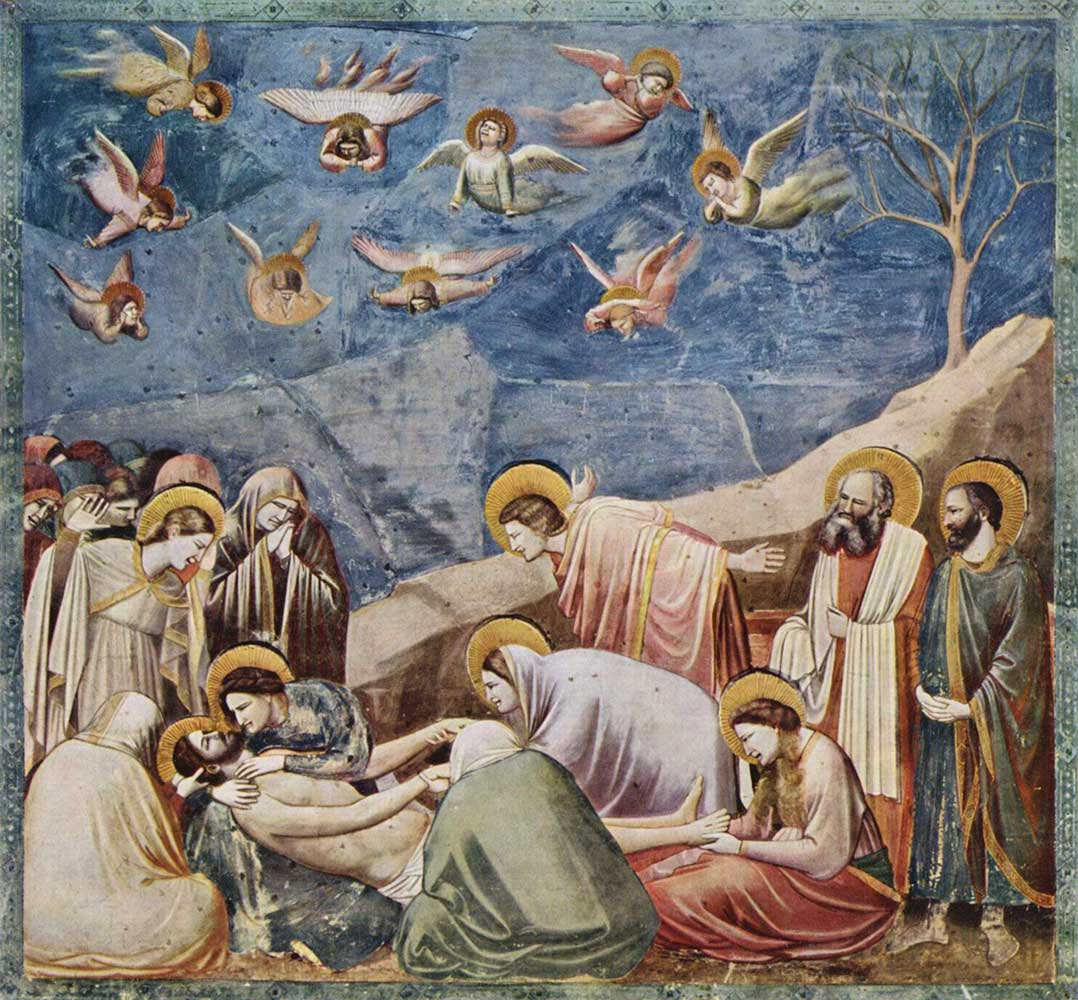
\includegraphics[width=0.8\textwidth]{./04-figuras/giotto_lamentacao}
    \label{fig:giotto_lamentacao}
\end{figure}
\vspace*{-0,9cm}
{\raggedright \fonte{\citeonline{muga}}}\\

\citeonline{muga} relata que é a partir do renascimento que o paradigma da luz atributo dá lugar ao da luz efeito. Além disso, conclui que foi mergulhando na \textit{camara oscura} que vários pintores do barroco e do renascimento perseguiram uma representação realista da natureza. E que, graças à ela Leonardo da Vinci desenvolveu o método \textit{chiaroscuro} e o \textit{sfumato}, reforçando a tridimensionalidade e a profundidade da representação, evidenciando, assim, o efeito da luz incidente e das partículas atmosféricas na difusão da luz. Esse estudo,  como podemos ver na figura \ref{fig:da_vinci_virgem_rochedos}, \textit{A virgem dos rochedos} de Leonardo da Vinci, é desenvolvido no seio da escuridão que antes atributo do mal, torna-se aliada para se chegar à luz, afirma \citeonline{muga}.

\begin{figure}[H]
    \centering
    \caption{\textit{A virgem dos rochedos} (1495-1508), Leonardo da Vinci}
	\vspace*{0,2cm}
    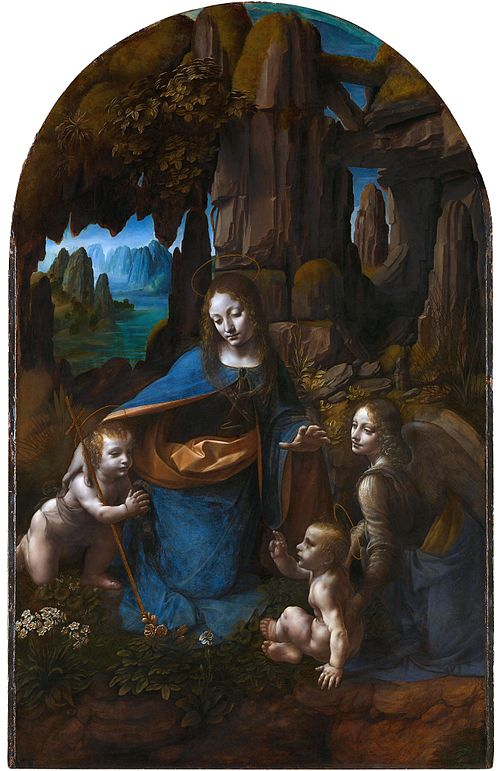
\includegraphics[width=0.4\textwidth]{./04-figuras/da_vinci_virgem_rochedos}
    \label{fig:da_vinci_virgem_rochedos}
\end{figure}
\vspace*{-0,9cm}
{\raggedright \fonte{\citeonline{muga}}}\\


Com o advento da fotografia os pintores precisaram se reinventar. Para \citeonline[p. 77]{henno} "o progresso tecnológico atrelado a fotografia exigiu que os artistas deslocassem o hábito descritivo da mimesis para um desenvolvimento interno de sua criatividade". Voltando a \citeonline{muga}, a fotografia influenciou os impressionistas a saírem do ateliês e procurarem no interior do globo ocular a percepção de uma natureza que, a cada mutação de luz, mudava de aspecto e de verdade. Segundo \apudonline{gombrich}{muga} Édouard Manet e seus seguidores descobriram que "ao olharmos a natureza ao ar livre e à plena luz do dia, as formas redondas parecem planas, e não vemos os objetos cada um com a sua cor própria, mas uma mistura brilhante de matizes que se combinam nos nossos olhos".


De acordo com \citeonline[p. 78]{henno} foi apoiado no preceito de que a cor se mistura no olho e não na paleta que Seurat aplicava pontos de cor na tela, em locais estratégicos, a fim de que a mistura desses pontos, a partir de uma distância apropriada, fossem vistos como uma única cor pelo observador. Na figura \ref{fig:seurat_la_parede} podemos ver a obra  \textit{La Parede} do artista e na figura \ref{fig:seurat_la_parede_detalhe} um detalhe ampliado desta mesma obra, que nos faz perceber como a mesma é constituída.

\begin{figure}[H]
    \centering
    \caption{\textit{La Parade} (1887-88), Georges Seurat}
	\vspace*{0,2cm}
    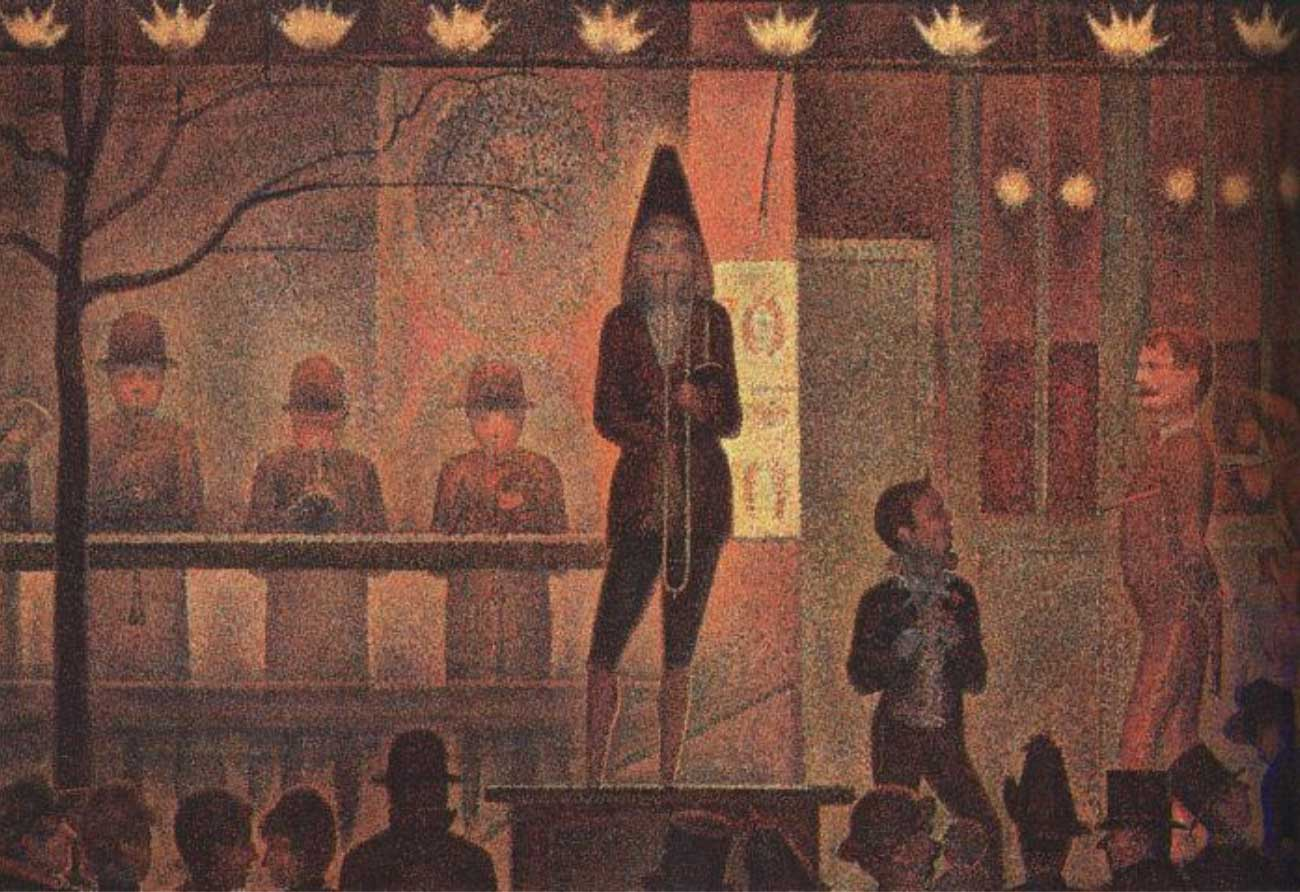
\includegraphics[width=0.8\textwidth]{./04-figuras/seurat_la_parede}
    \label{fig:seurat_la_parede}
\end{figure}
\vspace*{-0,9cm}
{\raggedright \fonte{\citeonline[p.79]{henno}}}\\
   
\begin{figure}[H]
    \centering
    \caption{\textit{La Parade} (1887-88) - detalhe ampliado, Georges Seurat}
	\vspace*{0,2cm}
    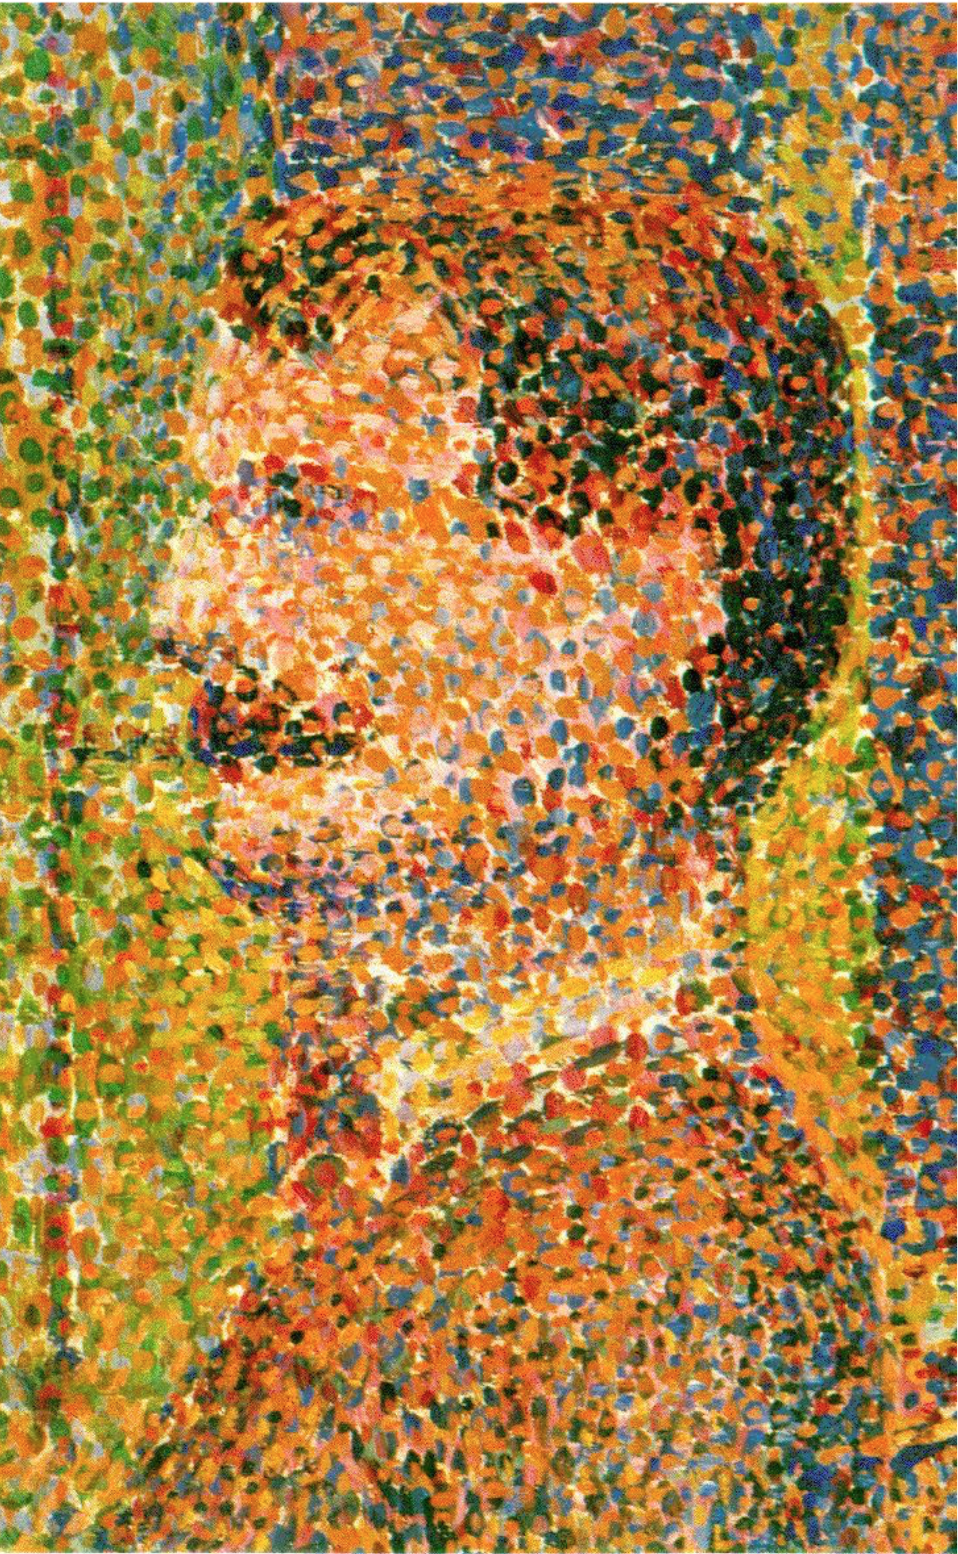
\includegraphics[width=0.4\textwidth]{./04-figuras/seurat_la_parede_detalhe}
    \label{fig:seurat_la_parede_detalhe}
\end{figure}
\vspace*{-0,9cm}
{\raggedright \fonte{\citeonline[p.79]{henno}}}\\

Para \citeonline{muga}, depois de ocupar o lugar de atributo brilhante e de efeito de iluminação, ao longo so século XX, a luz se torna um meio. Segundo \citeonline[p. 1]{azevedo} a função da luz não é mais somente de iluminar, de tornar visível uma obra ou um objeto, ou o mero reflexo dos seus efeitos suspensos no espaço. A luz passa a ser tratada como objeto ou material. Na perspectiva da arte contemporânea, se vê que, em muitas obras, a luz passa à matéria. \citeonline[p. 23]{vega} afirma que, atualmente, muitos artistas exploram as possibilidades da luz artificial, trabalhando com mescla de materiais e diversos tipos de fontes de luz. \citeonline[p. 50]{brandi} destaca que "alguns artistas e movimentos estéticos estão fortemente relacionados com a linguagem da luz, mesmo quando não a utilizam como objeto central da obra". 


James Turrell, por exemplo, foi pioneiro de uma nova preocupação com os fenômenos do espaço e da luz. Em seus primeiros trabalhos investigou os efeitos da luz artificial. Ele também desenvolveu várias instalações que aumentaram a relação entre a luz e a estrutura arquitetônica. Em conversa com \citeonline[p. 114]{adcock}, ele relata que uma das dificuldades de usar a luz é que ainda não é tradição utilizá-la em nossa cultura. Por outro lado, não é mais incomum usá-la do que usar pedra, argila, aço ou tinta. O artista declara seu interesse em trabalhar a luz como material, mas não luz em vidro, fibra de vidro ou acrílico, e sim no próprio espaço e nas qualidades do espaço, fazendo luz sem a forma física tradicional. Ele nos traz também que há uma rica tradição na pintura do trabalho sobre a luz, mas que isso de fato não é luz - é o registro da visão. Na figura \ref{fig:james_turrell} podemos ver sua obra entitulada \textit{The light inside} que transforma as paredes de um túnel em vasos para a condução da luz e nos dá uma ideia da dimensão na qual o artista trabalha este material. 

\begin{figure}[H]
    \centering
    \caption{\textit{The light inside} (1999), James Turrell}
	\vspace*{0,2cm}
    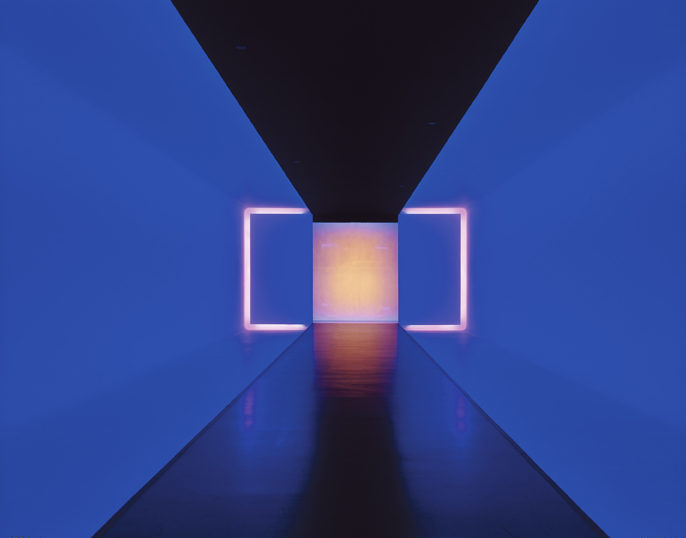
\includegraphics[width=0.8\textwidth]{./04-figuras/james_turrell}
    \label{fig:james_turrell}
\end{figure}
\vspace*{-0,9cm}
{\raggedright \fonte{Disponível em: <http://jamesturrell.com/work/thelightinside/>. Acesso em: 18 jun. 2018}}\\

Já o trabalho de Jim Campbell chama à atenção pela antítese presente em suas obras. Em um vídeo produzido pela \citeonline{kqed}, o artista constata que em um mundo de alta definição e telas cada vez mais finas usa tecnologia para produzir o contrário: imagens borradas e em baixa resolução em painéis tridimensionais. Não há projeção. Essas vídeo-esculturas (figura \ref{fig:jim_campbell}) são compostas por grades de LEDs que atuam como uma televisão de pixels desconstruída. De perto, as luzes piscam de maneira desordenada, sendo apenas uma constelação de pontos brilhantes sem muito significado. A peça só começa a se revelar quando o espectador se afasta, tornando-se primeiro uma uma onda sincronizada de luzes em movimento depois se transformando em imagens de crianças brincando ou homens e mulheres caminhando. 

\begin{figure}[H]
    \centering
    \caption{\textit{Light Topography Wave} (2014), Jim Campbell}
	\vspace*{0,2cm}
    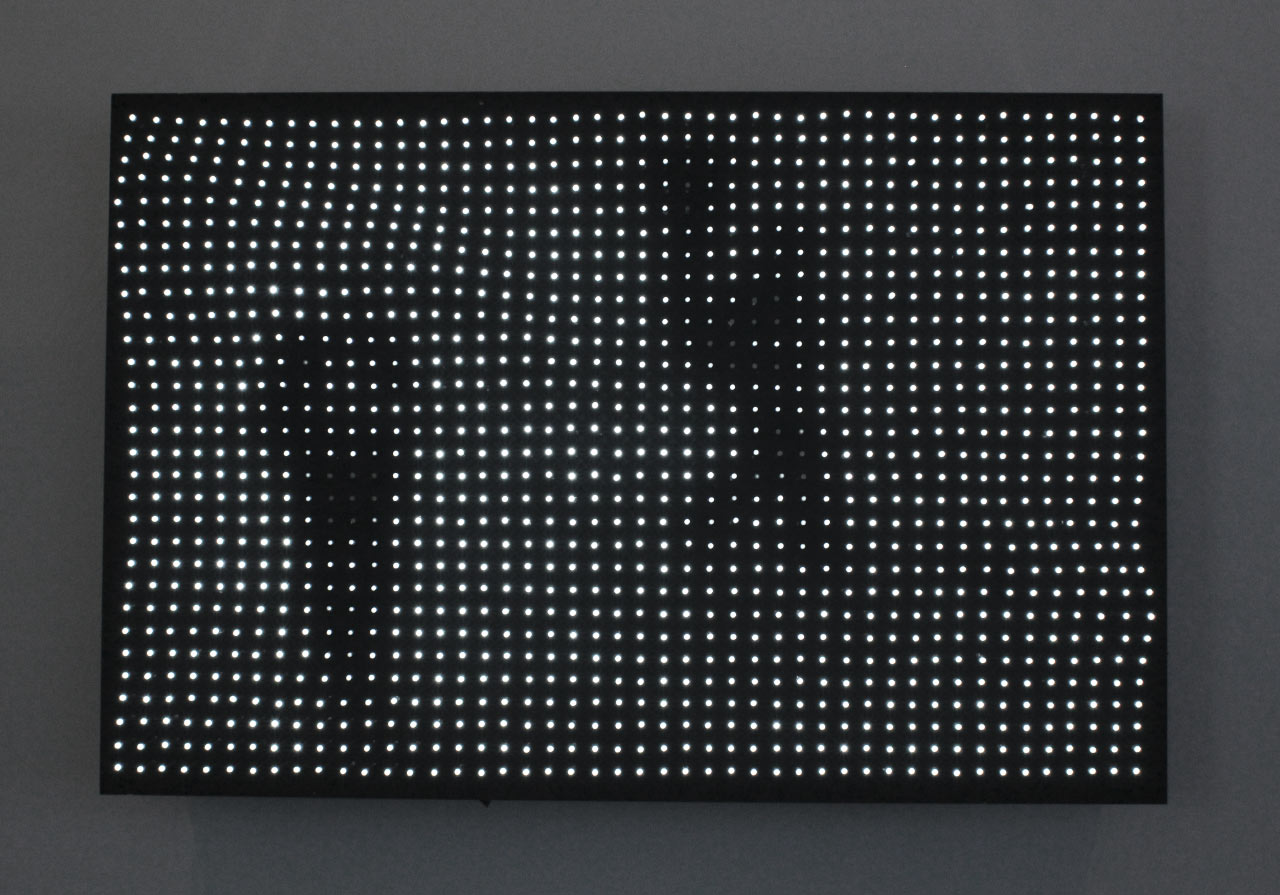
\includegraphics[width=0.8\textwidth]{./04-figuras/jim_campbell}
    \label{fig:jim_campbell}
\end{figure}
\vspace*{-0,9cm}
{\raggedright \fonte{Disponível em: <https://design-milk.com/pixelated-led-art-jim-campbell/>. Acesso em: 22 mar. 2018}}\\


\section{LUZ E INTERATIVIDADE}

\citeonline[p. 73]{henno} afirma que, aliado ao desenvolvimento da ciência e da tecnologia, o homem de hoje tem condições de gerar e projetar a luz artificialmente ao invés de se restringir aos meios naturais. E que, ao se apropriar da luz, o homem controla as emissões cromáticas a ela vinculadas, a partir de filtros ou de dispositivos tecnológicos específicos. Além disso, relata que o artista de hoje dispõe de ferramentas que lhe possibilitam projetar através da luz. E, dessa forma, no caso da luz como fonte de emissão ou projeção, o artista controla os dispositivos de luz, trabalhando poeticamente no momento em que confere um sentido à sua obra. Com o passar dos anos, os limites destes dispositivos se dissipam o que permite a interação homem e luz cada vez mais próxima. O reflexo dessa relação cada vez maior com os dispositivos técnicos, propicia uma abertura crescente da obra: o artista pode trabalhar em conjunto com o espectador na construção de seu sentido.


Um bom exemplo desta interação é a obra \textit{Optone} (figura \ref{fig:tsutomu_mutoh}), de autoria do designer Tsutomu Mutoh, que de acordo com \citeonline[p. 115]{henno}, usa um objeto com um eixo vertical que, em seu topo, possui uma cúpula contendo LEDs que se iluminam a partir do movimento aplicado pelo interator. Devido a seu peso e à ação da gravidade, a cúpula, pode ser movimentada sem que a base perca o contato com o solo. Assim, movimentos de rotação e balanço feitos por quem interage com o objeto são detectados por sensores, acionando os LEDs que estão dentro da cúpula. Ambos os dispositivos estão vinculados a um \textit{software}, desenvolvido pelo autor, que associa uma cor às coordenadas pelas quais a cúpula passa.

\begin{figure}[H]
    \centering
    \caption{\textit{Optone} (2009), Tsutomu Mutoh}
	\vspace*{0,2cm}
    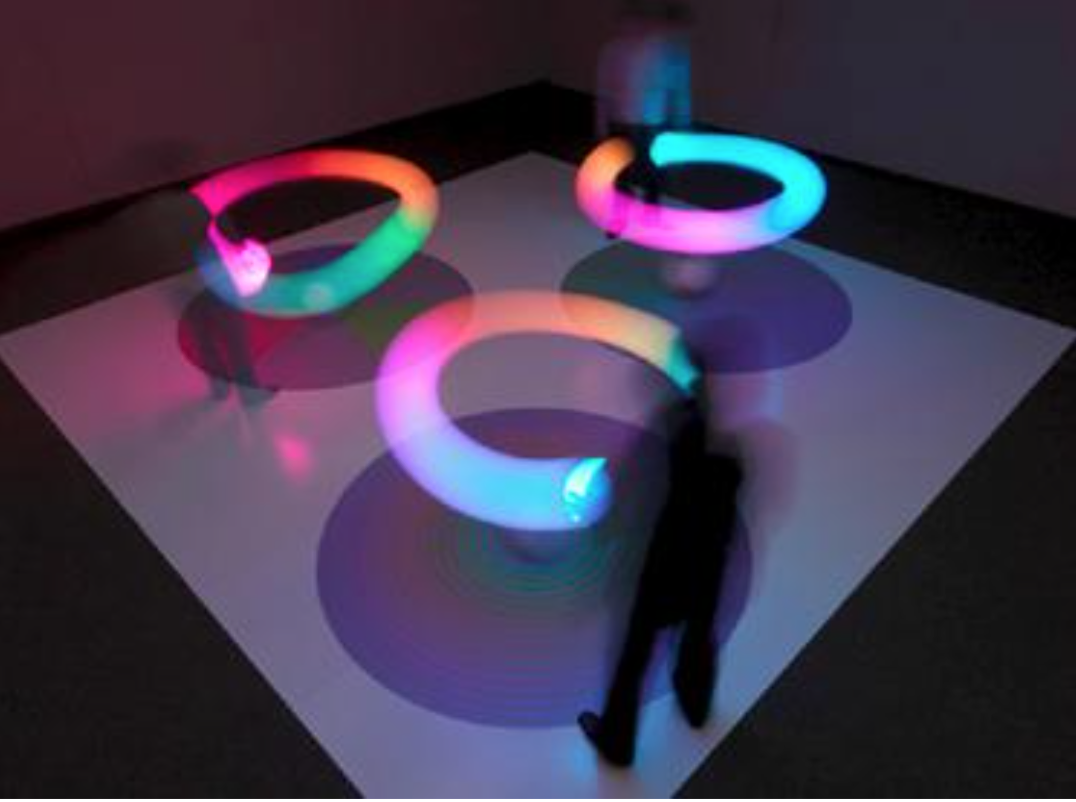
\includegraphics[width=0.8\textwidth]{./04-figuras/tsutomu_mutoh}
    \label{fig:tsutomu_mutoh}
\end{figure}
\vspace*{-0,9cm}
{\raggedright \fonte{\citeonline[p. 115]{henno}}}\\

Outro artista cuja obra é relevante no contexto deste trabalho e que, além da luz, explora a perspectiva da arte computacional, é o japonês Takahito Matsuo que, segundo \citeonline[p. 5]{soares}, cria mundos interativos de fantasia e de luz que fazem parte de uma estética enigmática, misturando som e luz perante os movimentos do observador. Seu trabalho destaca as diferentes gradações de luz e sombra que contrastando mostram um mundo de fantasia e imaginação. Em \textit{Fantasias Aquáticas Iluminadas} (figura \ref{fig:takahito_matsuo}), a exploração através de luz, projeções, arquitetura e interações humanas é fortemente encorajada. À medida que os visitantes se aproximam das paredes, se movimentam e se afastam, o número e a frequência das medusas aumentam e diminuem. As formas orgânicas e a brilhante paleta de azúis criam um mundo subaquático surreal, onde movimentos lúdicos e interações com o espaço arquitetônico resultam em uma comunicação não dita entre artista e participante. 

\begin{figure}[H]
    \centering
    \caption{\textit{Fantasias Aquáticas Iluminadas} (2009), Takahito Matsuo}
	\vspace*{0,2cm}
    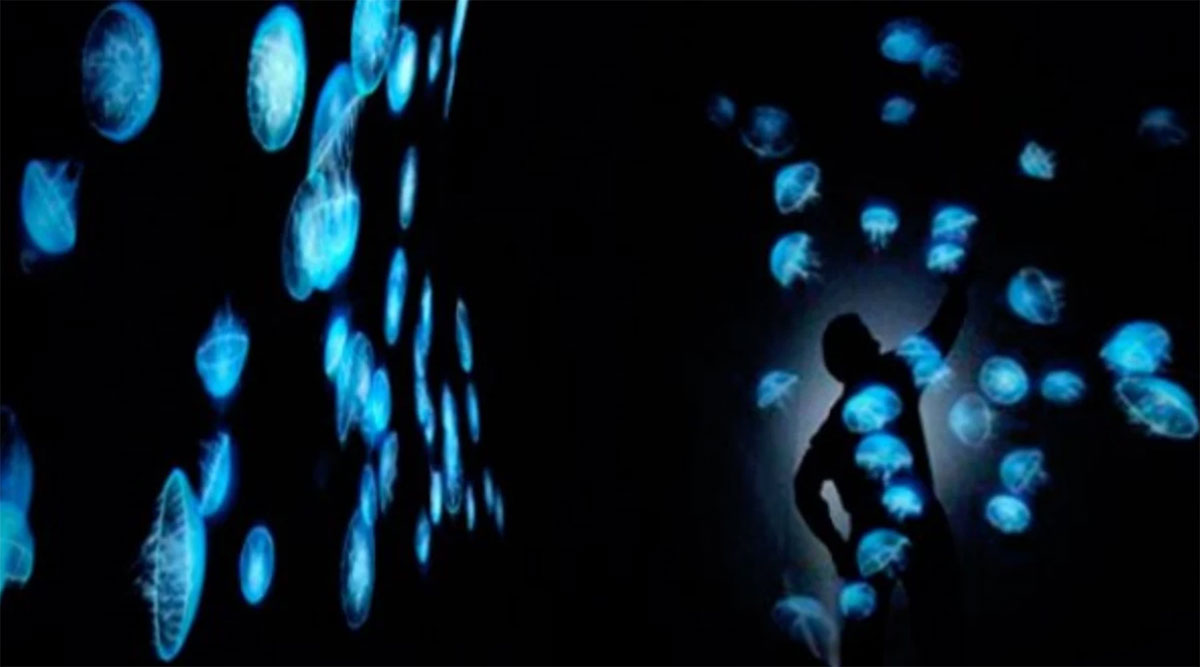
\includegraphics[width=0.8\textwidth]{./04-figuras/takahito_matsuo}
    \label{fig:takahito_matsuo}
\end{figure}
\vspace*{-0,9cm}
{\raggedright \fonte{\citeonline{soares}}}\\


\section{O CUBO PRETO}

O cubo branco tende a não ser o cenário ideal para exibição de obras que tem a luz como material. \citeonline[p. 40]{soares}, afirma que "a maioria dos autores que trabalham com arte e tecnologia procuram o espaço do cubo preto como espaço expositivo. Neste espaço o que interessa é um novo ver, um espanto com a imagem". Diz ainda que o nome cubo preto para este tipo de exposição surge em contraposição ao cubo branco, criado por Brian O'Doherty, num ensaio publicado pela revista Artforum em 1976, fazendo alusão ao espaço das galerias de arte, com paredes brancas, sem janelas isolando o espetador num meio aparentemente atemporal. A ideia do cubo preto surge como ambiente ideal para propagação da luz e é também uma forma de imersão no interior da mente do artista.

De acordo com \citeonline[p. 63]{sogabe2011} quando pensamos em instalações interativas, temos a lembrança de uma sala fechada e escura. Ele diz que essa condição está relacionada ao tipo de projetores de imagens existentes em uma época, com baixa luminosidade e que necessitavam de escuridão para apresentarem imagens nítidas. O autor afirma que, atualmente, essa condição já não é obrigatória, pois temos projetores de alta luminância, que podem funcionar em ambientes totalmente iluminados. Conclui então que, pela melhora dos equipamentos, o ambiente escuro passa a ser uma opção e não uma condição necessária. Ainda que isso possa ser verdade no que tange à imagem projetada, quando se trata da luz como fonte de emissão não se pode dizer o mesmo. \citeonline[p. 125]{henno} afirma que quando há pouca ou nenhuma luminosidade, a intensidade das cores é maior e mais perceptível devido ao contraste com a escuridão. E, além disso, o contraste da cor como informação luminosa em face da escuridão estabelece comunicação com o observador seduzindo-o pelos sentidos que tal cor suscita.

           	% Ilustrações
    \chapter{COMPOSIÇÃO DA OBRA}
Esta capítulo está organizado em quatro partes. Primeiro vamos trazer um breve relato sobre os dispositivos e tecnologias utilizados, depois apresentaremos o protótipo construído para validar o \textit{software} e o \textit{hardware} escolhidos para elaboração da obra, em seguida vamos fazer uma descrição da solução, apresentando as principais barreiras encontradas ao longo do percurso e, por fim, apresentaremos o projeto de instalação e montagem. 

\section{DISPOSITIVOS E TECNOLOGIAS}

Com o intuito de manter documentada, possibilitando a reprodução ou atualização deste projeto no futuro, se faz necessário listar as versões e configurações aplicadas (quadro \ref{quadro:dispositivos}), bem como introduzir os principais dispositivos e tecnologias utilizados. Dentre os componentes essenciais em termos de \textit{hardware} temos o Microsoft Kinect, o Arduino e o computador; enquanto o principal \textit{software} é a Processing, responsável por orquestrar o funcionamento destes equipamentos em conjunto, através de um \textit{script} desenvolvido ao longo desse trabalho. 


\begin{quadro}[H]
\caption{\label{quadro:dispositivos}Especificações de \textit{hardware} e \textit{software} utilizados}
\begin{center}  
  \begin{tabulary}{0.8\textwidth}{|L|L|}
  
  \hline
  \textbf{Dispositivo ou \textit{software}} & \textbf{Requisitos} \\ \hline
  Microsoft Kinect  & Versão 1 - Modelo 1414 \\ \hline
  Arduino & Modelo Uno para o protótipo e Modelo Mega 2560 para o trabalho final \\ \hline
  Computador & Suporte a versão da Processing utilizada e disponibilidade de 2 portas USB \\ \hline
  Processing & Versão 3.3.7 \\ \hline
  \end{tabulary}
\end{center}
\vspace*{-0,7cm}
\fonte{Elaborado pela autora}\\
\end{quadro}


A figura \ref{fig:dispositivos} mostra como esses dispositivos estão interligados: o Kinect envia dados de profundidade para o computador, que através de um programa escrito em Processing, realiza cálculos e processamento das informações recebidas e, em seguida, envia instruções para o Arduino. Esse processo é cíclico e constante durante toda a execução da obra.

\begin{figure}[H]
  \begin{center}
    \caption{Dispositivos utilizados na construção da obra}
    \vspace*{0,2cm}
    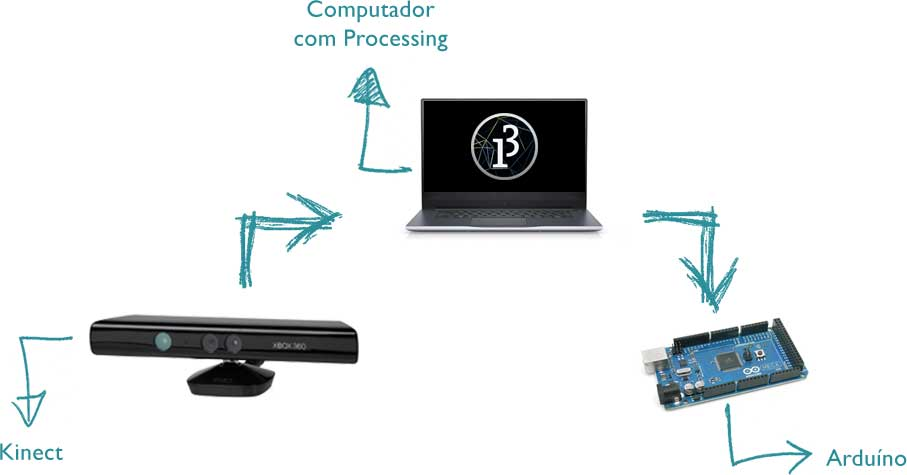
\includegraphics[width=0.8\textwidth]{./04-figuras/dispositivos}
    \label{fig:dispositivos}
  \end{center}
  \vspace*{-0,9cm}
  \fonte{Elaborada pela autora}\\
\end{figure}


\subsection{Microsoft Kinect}

O sensor Kinect é um dispositivo lançado em 4 de Novembro de 2010 como um acessório do console Xbox 360 da Microsoft. Orientado, principalmente, a indústria de jogos, foi criado para servir como uma forma de interação entre o utilizador e o console Xbox 360 através de gestos e comandos de voz. De acordo com a \citeonline{microsoft}, em sua primeira versão, é capaz de capturar imagens com 640x480 \textit{pixels} a 30 fps. O aparelho é formado por um emissor e sensor de profundidade baseados em infravermelho, uma câmera RGB, um motor de inclinação e uma série de 4 microfones. Na figura \ref{fig:kinect_componentes} podemos ver a posição de cada um destes componentes no dispositivo.

\begin{figure}[H]
  \begin{center}
    \caption{Componentes do sensor Kinect}
    \vspace*{0,2cm}
    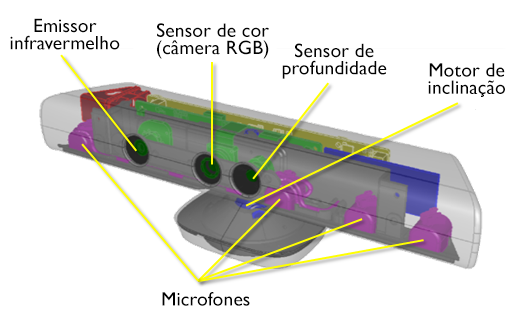
\includegraphics[width=0.8\textwidth]{./04-figuras/kinect_componentes}
    \label{fig:kinect_componentes}
  \end{center}
  \vspace*{-0,9cm}
  \fonte{Adaptado de \citeonline{microsoft}}\\
\end{figure}

Dentre seus componentes, o que mais nos interessa no contexto deste trabalho, é o sensor de profundidade. \citeonline{ashley} afirmam que a produção de dados tridimensionais é a principal função do Kinect. Ele difere de qualquer outro dispositivo de entrada justamente porque provê uma terceira dimensão e, para tanto, se utiliza de um emissor e uma câmera de infravermelho. Segundo \citeonline{lucero} o emissor projeta um padrão estruturado de luz infravermelha, enquanto a câmera lê esses raios e interpreta a deformação da projeção, convertendo essa informação em valores de profundidade e, consequentemente, medindo a distância entre o objeto e o sensor. De acordo com \citeonline{correia} estas medidas baseiam-se em triangulação tendo em conta o emissor, a câmera e as posições dos \textit{pixels} no cenário. A profundidade é codificada numa escala de cinzas. Quanto mais escuro o \textit{pixel}, mais próximo do sensor está esse ponto no espaço. Sendo que, \textit{pixels} pretos indicam que não existe informação de profundidade. Isto ocorre no caso dos pontos estarem muito longe, impossibilitando a sua captura, no caso de estarem numa área onde não haja pontos do emissor de infravermelhos, no caso de o objeto refletir mal a luz infravermelha ou, finalmente, no caso de os pontos estarem muito próximos do sensor, uma vez que o campo de visão do Kinect é limitado em cerca de 80 centímetros a 4 metros.

\subsection{Arduino}

O Arduino é uma plataforma de prototipação eletrônica de \textit{hardware} livre e de placa única \cite{arduino}. De acordo com o \textit{site} oficial do projeto, o objetivo é criar ferramentas acessíveis, com baixo custo, flexíveis e fáceis de usar. Para \citeonline{souza2011} ela é ideal para a criação de dispositivos que permitam interação com o ambiente, podendo utilizar diversas fontes de entrada como, por exemplo, sensores de temperatura, luz ou som, e como saída LEDs, motores, \textit{displays}, auto-falantes, entre outros, criando desta forma possibilidades ilimitadas. É possível dizer à placa o que fazer enviando uma série de instruções ao microcontrolador. Para isso é necessário utilizar a linguagem de programação do Arduino (baseada em Wiring) e o seu \textit{software} (IDE - \textit{Integrated Development Environment} ou Ambiente de Desenvolvimento Integrado), baseada em Processing \cite{arduino}. 


\subsection{Processing}
\label{sec:processing}

De acordo com \citeonline[p. 115]{santos} Processing é a primeira ferramenta criada para artistas por artistas e o seu desenvolvimento foi iniciado no MIT Media Lab por dois estudantes de graduação: Casey Reas e Benjamin Fry. Segundo informações contidas no \textit{site} oficial do projeto, \citeonline{processing} é uma plataforma e uma linguagem de programação de código aberto (\textit{open source}) para prototipação de \textit{software} dentro do contexto das artes visuais. Disponível desde 2001, a Processing vem promovendo a alfabetização em \textit{software} dentro das artes visuais e a alfabetização visual dentro da tecnologia. 

\subsection{Computador}
\label{sec:computador}

Este trabalho requer a utilização de um computador para processar os dados capturados pelo Kinect e enviar ao Arduino. O projeto foi desenvolvido e testado em equipamentos com configurações distintas, sendo que, à princípio, seus únicos requisitos são o suporte à instalação da versão de Processing mencionada no quadro \ref{quadro:dispositivos}, disponível no início deste capítulo, e duas portas USB, uma para cada dispositivo. Não foram realizados testes de \textit{performance} para identificar a configuração mínima necessária para suportar o processamento de imagem executado. Estuda-se a possibilidade de utilização de um Raspberry PI (\citeyear{raspberry}), que é uma série de computadores de placa única que se conecta a um monitor e utiliza \textit{mouse} e teclado padrões, para obter como resultado uma instalação mais compacta e sem tantos dispositivos aparentes.



\section{PROTOTIPAÇÃO E TESTES}

Para validar o projeto foi construído um protótipo com o Microsoft Kinect, um computador, um Arduino Uno e 5 LEDs conectados à ele conforme pode ser visto na figura \ref{fig:prototipo}. Através da utilização de duas bibliotecas, \textit{Open Kinect for Processing} e Firmata, construiu-se um \textit{script} simplificado que controlava os dispositivos de entrada e saída de forma integrada, causando, assim, o acender e apagar dos LEDs de acordo com as informações capturadas pelo sensor. Desejava-se provar a possibilidade de, primeiro, controlar os dispositivos de entrada e saída de dados de maneira simultânea e, depois, a capacidade da luz emitida pelo LED se propagar através da fibra ótica.

\begin{figure}[H]
  \begin{center}
    \caption{Componentes do prótotipo}
    \vspace*{0,2cm}
    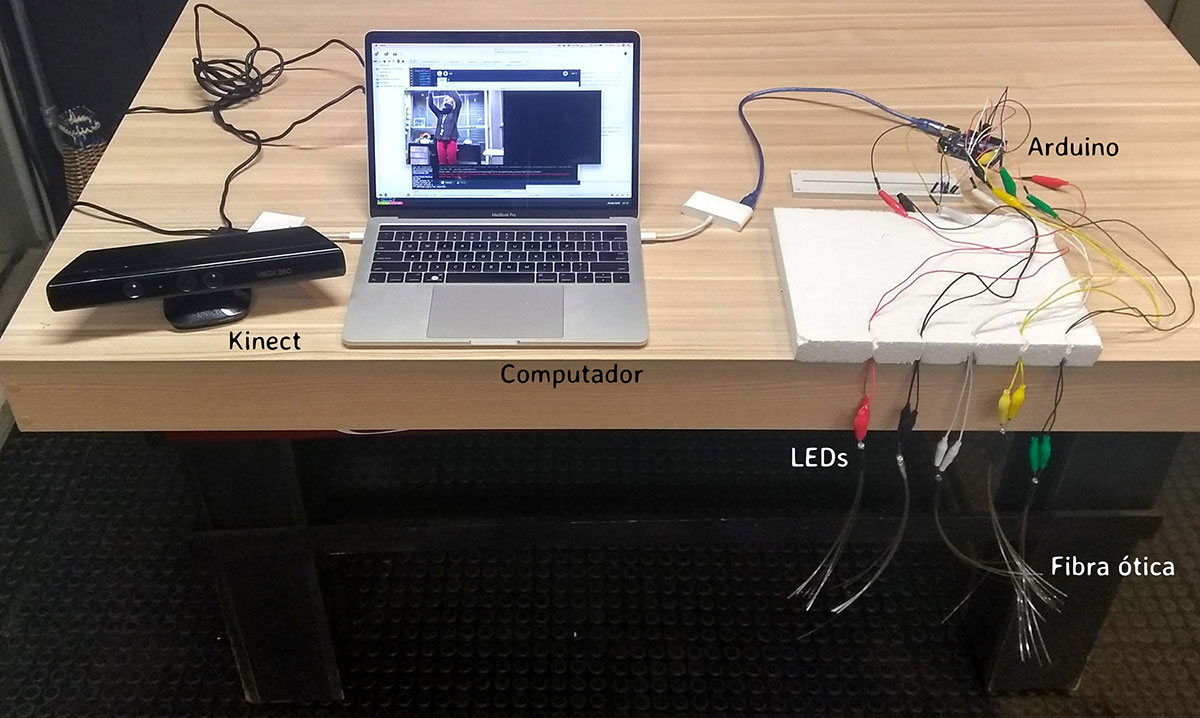
\includegraphics[width=0.8\textwidth]{./04-figuras/prototipo}
    \label{fig:prototipo}
  \end{center}
  \vspace*{-0,9cm}
  \fonte{Elaborada pela autora}\\
\end{figure}

No que diz respeito a integração dos elementos presentes na obra, foi possível constatar seu correto funcionamento já em conformidade com o modelo da proposta introduzida na \fullref{sec:solucao}, pois os dispositivos utilizados para prototipação são os mesmos ou muito similares aos que encontramos no trabalho final. A partir disso, o desafio se concentrou em construir a malha de LEDs, bem como fazer a colagem da fibra ótica em cada um deles, além de criar a versão final do \textit{script} que deveria funcionar como uma matriz e carecia de otimização em sua lógica de detecção de presença.

Na figura \ref{fig:prototipo_escuro} podemos ver uma amostra do protótipo sendo executado em um ambiente com baixa luminosidade. Constatou-se que a luz conseguia se propagar ao longo da fibra, mas que se mostrava com maior intensidade em suas extremidades. A partir disso foi elaborada uma proposta de junção dos LEDs com a fibra ótica que será apresentada mais adiante na  \fullref{sec:malha}.

\begin{figure}[H]
  \begin{center}
    \caption{Protótipo em ambiente com baixa luminosidade}
    \vspace*{0,2cm}
    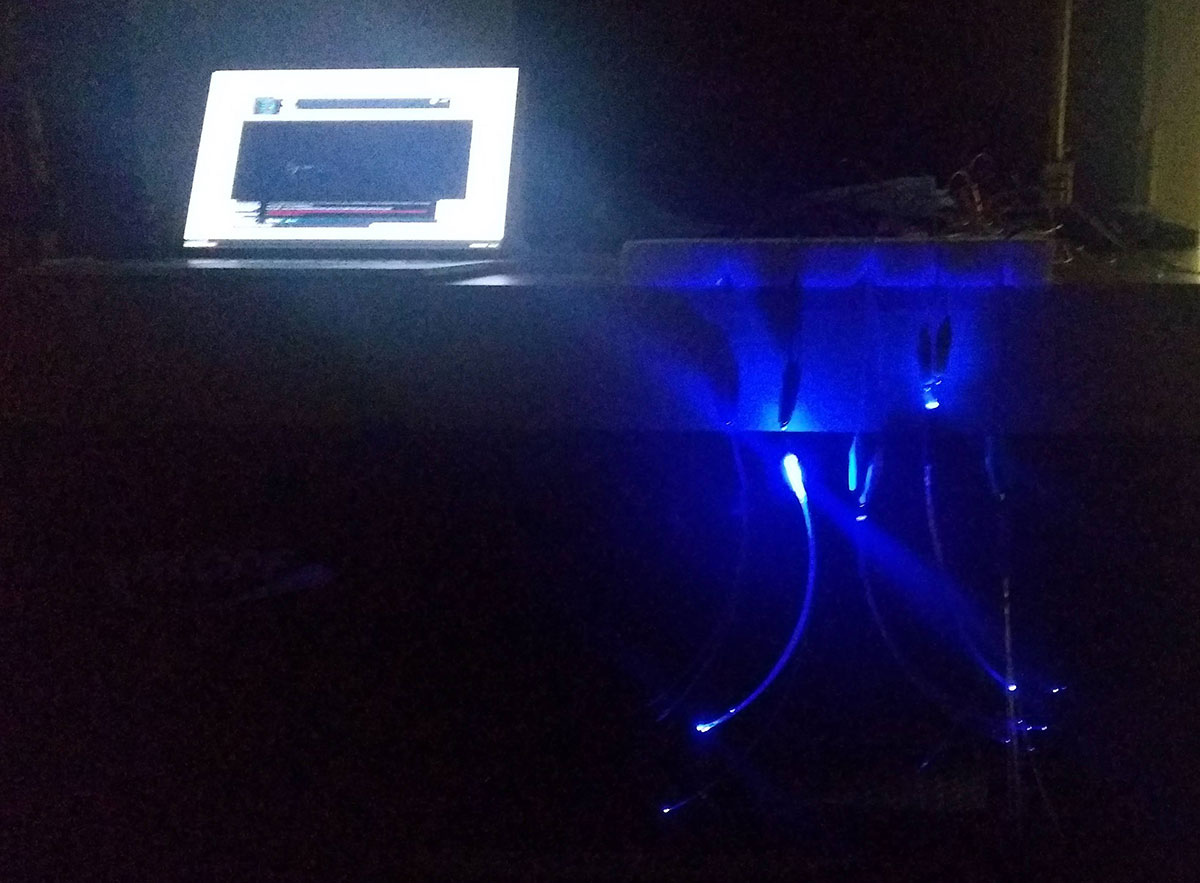
\includegraphics[width=0.8\textwidth]{./04-figuras/prototipo_escuro}
    \label{fig:prototipo_escuro}
  \end{center}
  \vspace*{-0,9cm}
  \fonte{Elaborada pela autora}\\
\end{figure}

\section{DESCRIÇÃO DA SOLUÇÃO}
\label{sec:solucao}

Para efeitos de organização e com o intuito de facilitar a compreensão, esta seção foi organizada de acordo com os elementos presentes no modelo de instalação interativa proposto por \citeonline{sogabe2011} já cobertos na \fullref{sec:instalacoes_interativas}. São eles: a interface, representada pelo sensor Microsoft Kinect, que parece invisível dado que o interator precisa apenas estar com o seu corpo presente no espaço para que a obra se materialize; o gerenciamento digital que é feito através de um computador e da utilização de Processing para execução e manutenção do programa; e, por fim, o dispositivo de saída de dados, aqui reprensentado por uma composição entre a malha de LEDs e o Arduino, traduzindo informação em luz.

Devido ao recurso de capturar objetos e movimentos no espaço, optou-se pelo uso do sensor Microsoft Kinect que, conectado a um computador, é responsável por captar a área onde os espectadores se encontram. Integrando-o a uma placa Arduino é possível controlar uma série de LEDs, dispostos em uma grade pendente ao teto. Cada LED possui cabos de fibra ótica \textit{side light} (com emissão de luz lateral) conectados à ele que se iluminam conforme os espectadores caminham sob a grade. Na figura \ref{fig:esquema} podemos ver um esquema de montagem da obra.

\begin{figure}[H]
  \begin{center}
    \caption{Esquema de montagem da obra}
    \vspace*{0,2cm}
    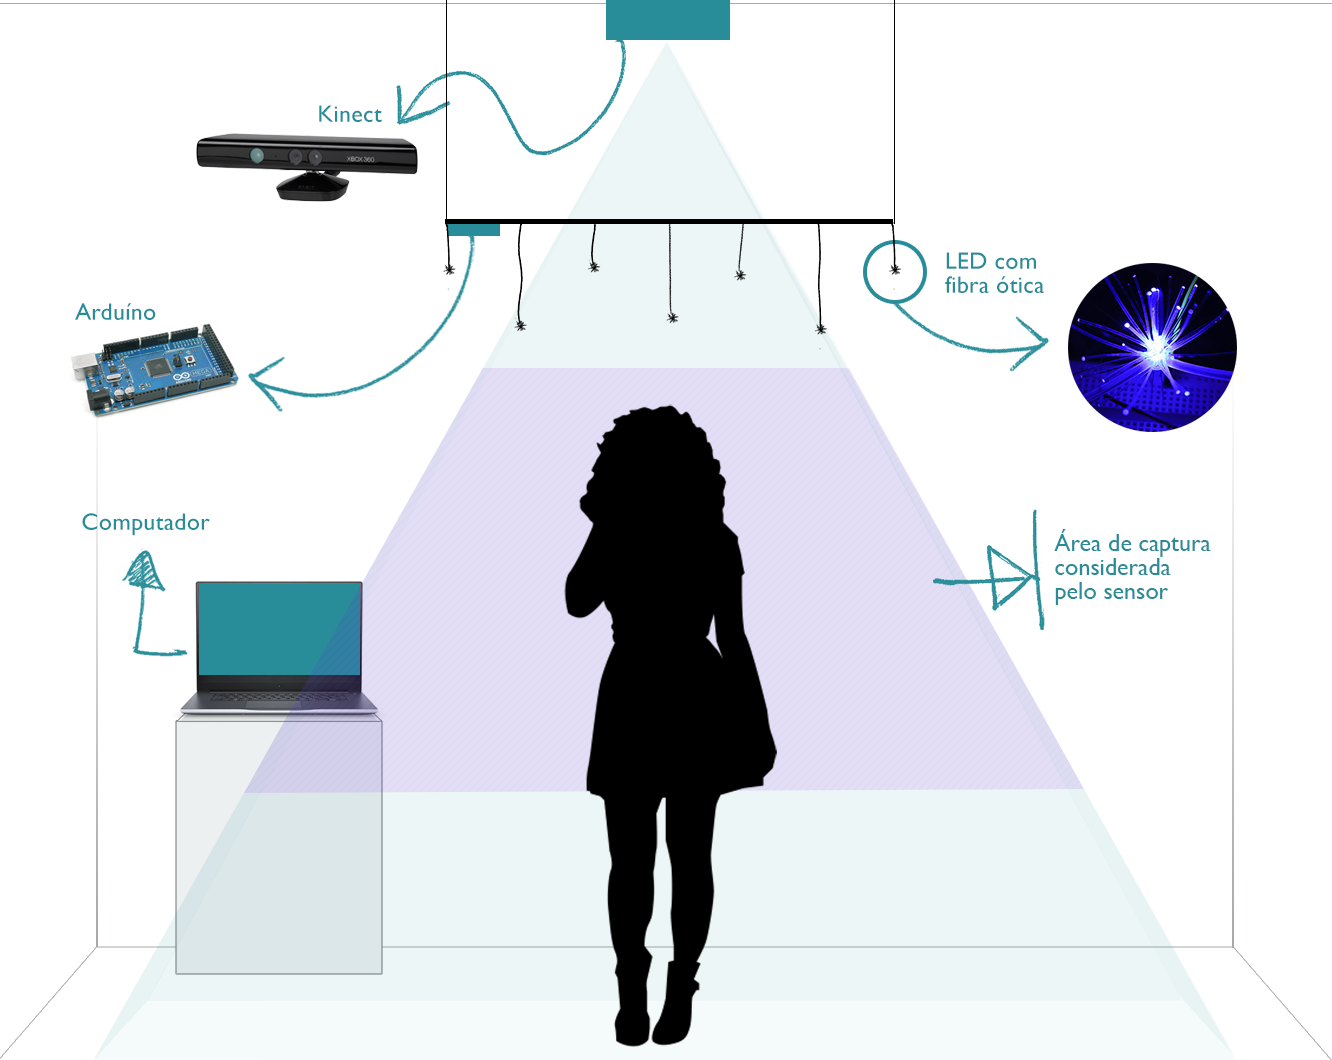
\includegraphics[width=0.8\textwidth]{./04-figuras/esquema}
    \label{fig:esquema}
  \end{center}
  \vspace*{-0,9cm}
  \fonte{Elaborada pela autora}\\
\end{figure}


\subsection{Interface}

O Microsoft Kinect atua como interface da instalação interativa proposta neste trabalho sendo utilizado como fonte de entrada de dados (\textit{input}) para mapear o ambiente tridimensional. Considerando suas limitações, a que mais impactou este projeto é causada pela própria natureza da luz projetada pelo sensor. A luz emitida pelo projetor de infravermelho, ao se deparar com um objeto, gera uma sombra em outro que esteja numa distância maior. Segundo \citeonline{lucero} o resultado é que não se pode determinar a profundidade em zonas afetadas por estas sombras, pois elas criam zonas negras na imagem de profundidade, ou seja, \textit{pixels} com valor zero, como pode ser visto na figura \ref{fig:kinect_sombras}. O impacto gerado aqui é devido à malha de LEDs se encontrar entre o Kinect e o interator. A malha projeta uma sombra, criando pontos onde a área de intersecção entre o LED e o espectador pode não ser percebida. Para contornar este problema, ao invés de um ponto específico, adotou-se uma região maior que a espessura da sombra para garantir o acendimento dos LEDs.

\begin{figure}[H]
  \begin{center}
    \caption{Efeito das sombras no sensor Kinect}
    \vspace*{0,2cm}
    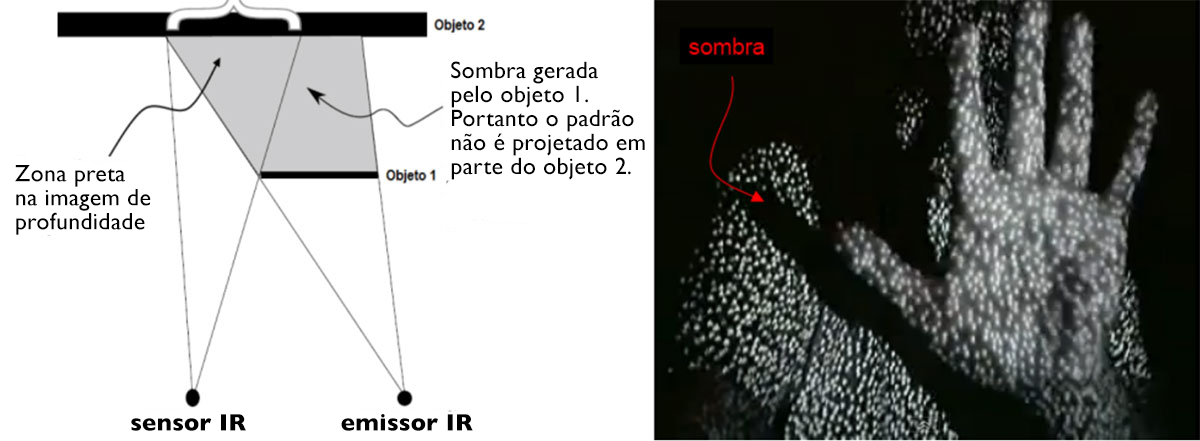
\includegraphics[width=0.8\textwidth]{./04-figuras/kinect_sombras}
    \label{fig:kinect_sombras}
  \end{center}
  \vspace*{-0,9cm}
  \fonte{Adaptado de \citeonline{lucero}}\\
\end{figure}

Além disso, o Kinect foi configurado através do \textit{script} para considerar a captura de objetos em uma área específica entre a grade e o solo, dessa maneira, apesar de não ser possível impedir a criação de sombras, conforme falado anteriormente, podemos, pelo menos, desconsiderar a grade como uma fonte de entrada de dados. A figura \ref{fig:kinect_exemplo} mostra dois exemplos de imagens criadas a partir dos dados capturados pelo sensor. À esquerda temos um caso sem a configuração mencionada e à direita uma imagem com o sensor já calibrado.

\begin{figure}[H]
  \begin{center}
    \caption{Imagens geradas a partir das informações capturadas pelo sensor Kinect}
    \vspace*{0,2cm}
    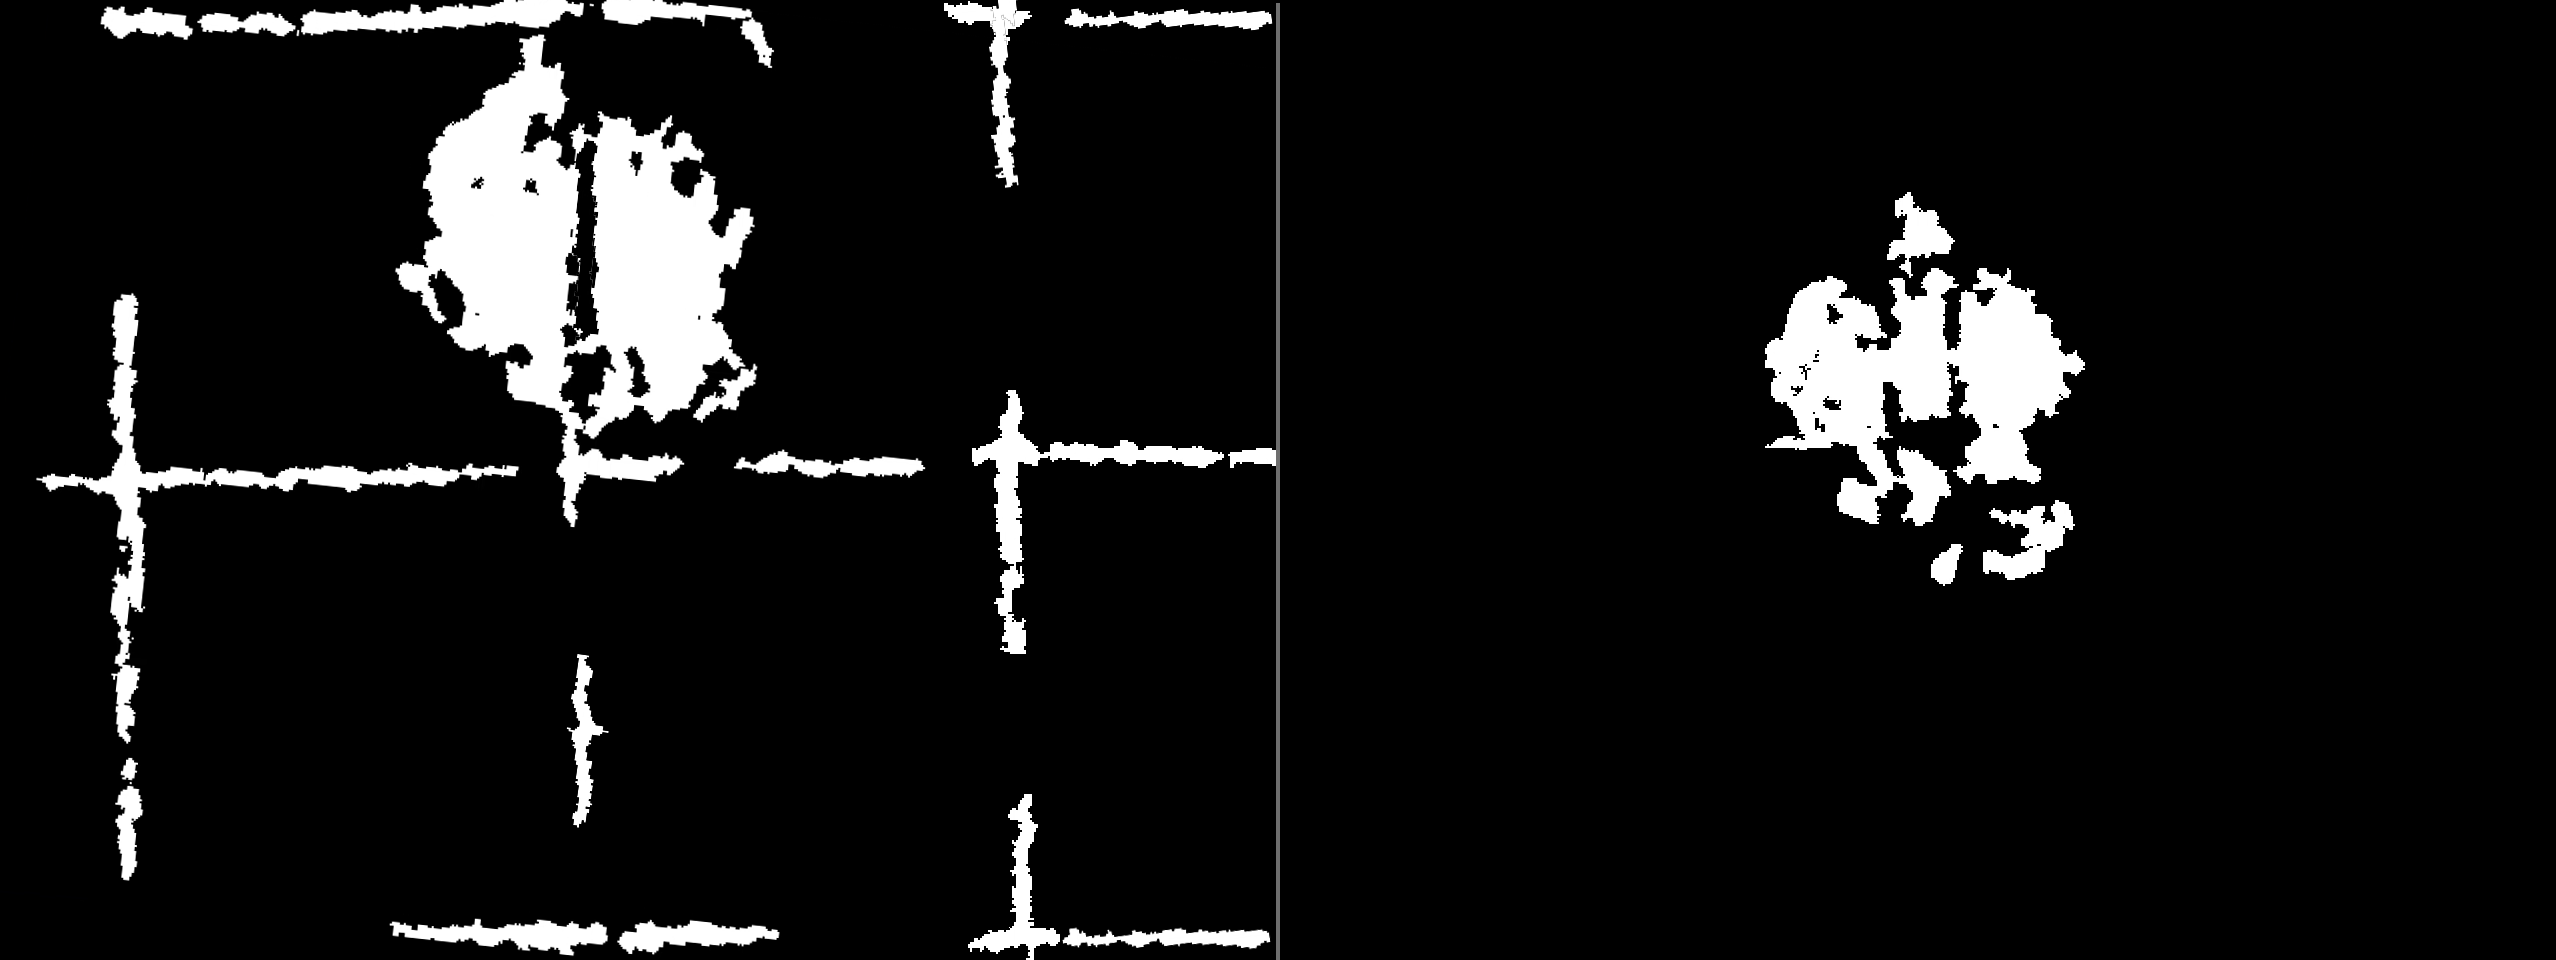
\includegraphics[width=0.8\textwidth]{./04-figuras/kinect_exemplo}
    \label{fig:kinect_exemplo}
  \end{center}
  \vspace*{-0,9cm}
  \fonte{Captura de tela gerada pelo sensor Kinect}\\
\end{figure}


Outro ponto importante que podemos observar na figura \ref{fig:kinect_exemplo} é que as imagens possuem apenas \textit{pixels} pretos e brancos. Este comportamento foi programado de maneira intencional. Isto porque, no âmbito desta proposta, nos interessa saber se existe algo (ou alguém) na área em questão e não a distância que possa estar da grade de LEDs. Dessa forma, interatores de diferentes estaturas podem criar o mesmo efeito ao caminhar sob a malha, ainda que, devido à diferença de distância do sensor, pessoas mais baixas pareçam menores na imagem capturada.


\subsection{Gerenciamento digital}

O gerencimento digital da obra é realizado através de um computador que executa um programa escrito em Processing. Interpretando as informações fornecidas pelo Kinect, por meio da biblioteca \textit{Open Kinect for Processing} e, gerando uma imagem bidimensional, que é utilizada por um algorítimo de detecção de cor, é possível determinar quais LEDs devem permanecer apagados e quais devem acender na estrutura. A figura \ref{fig:script} nos dá uma ideia de como o programa foi construído. À esquerda temos uma imagem da câmera com pontos brancos e pretos desenhados sobre ela, onde, cada um deles representa um LED na estrutura física. À direita temos a imagem gerada a partir dos dados do sensor de profundidade, sendo que as áreas brancas identificam a presença do interator. As coordenadas e área dos pontos que visualizamos na imagem à esquerda foram utilizados para capturar fragmentos na imagem à direita. A cor predominante no fragmento de imagem (branco ou preto) determina a informação que é enviada ao Arduino para que este, por fim, acenda ou apague os LEDs. Pontos brancos identificam os LEDs acesos, enquanto os pretos identificam os apagados.

\begin{figure}[H]
  \begin{center}
    \caption{Captura da câmera e imagem gerada a partir do sensor de profundidade associadas à pontos que identificam os LEDs na estrutura física}
    \vspace*{0,2cm}
    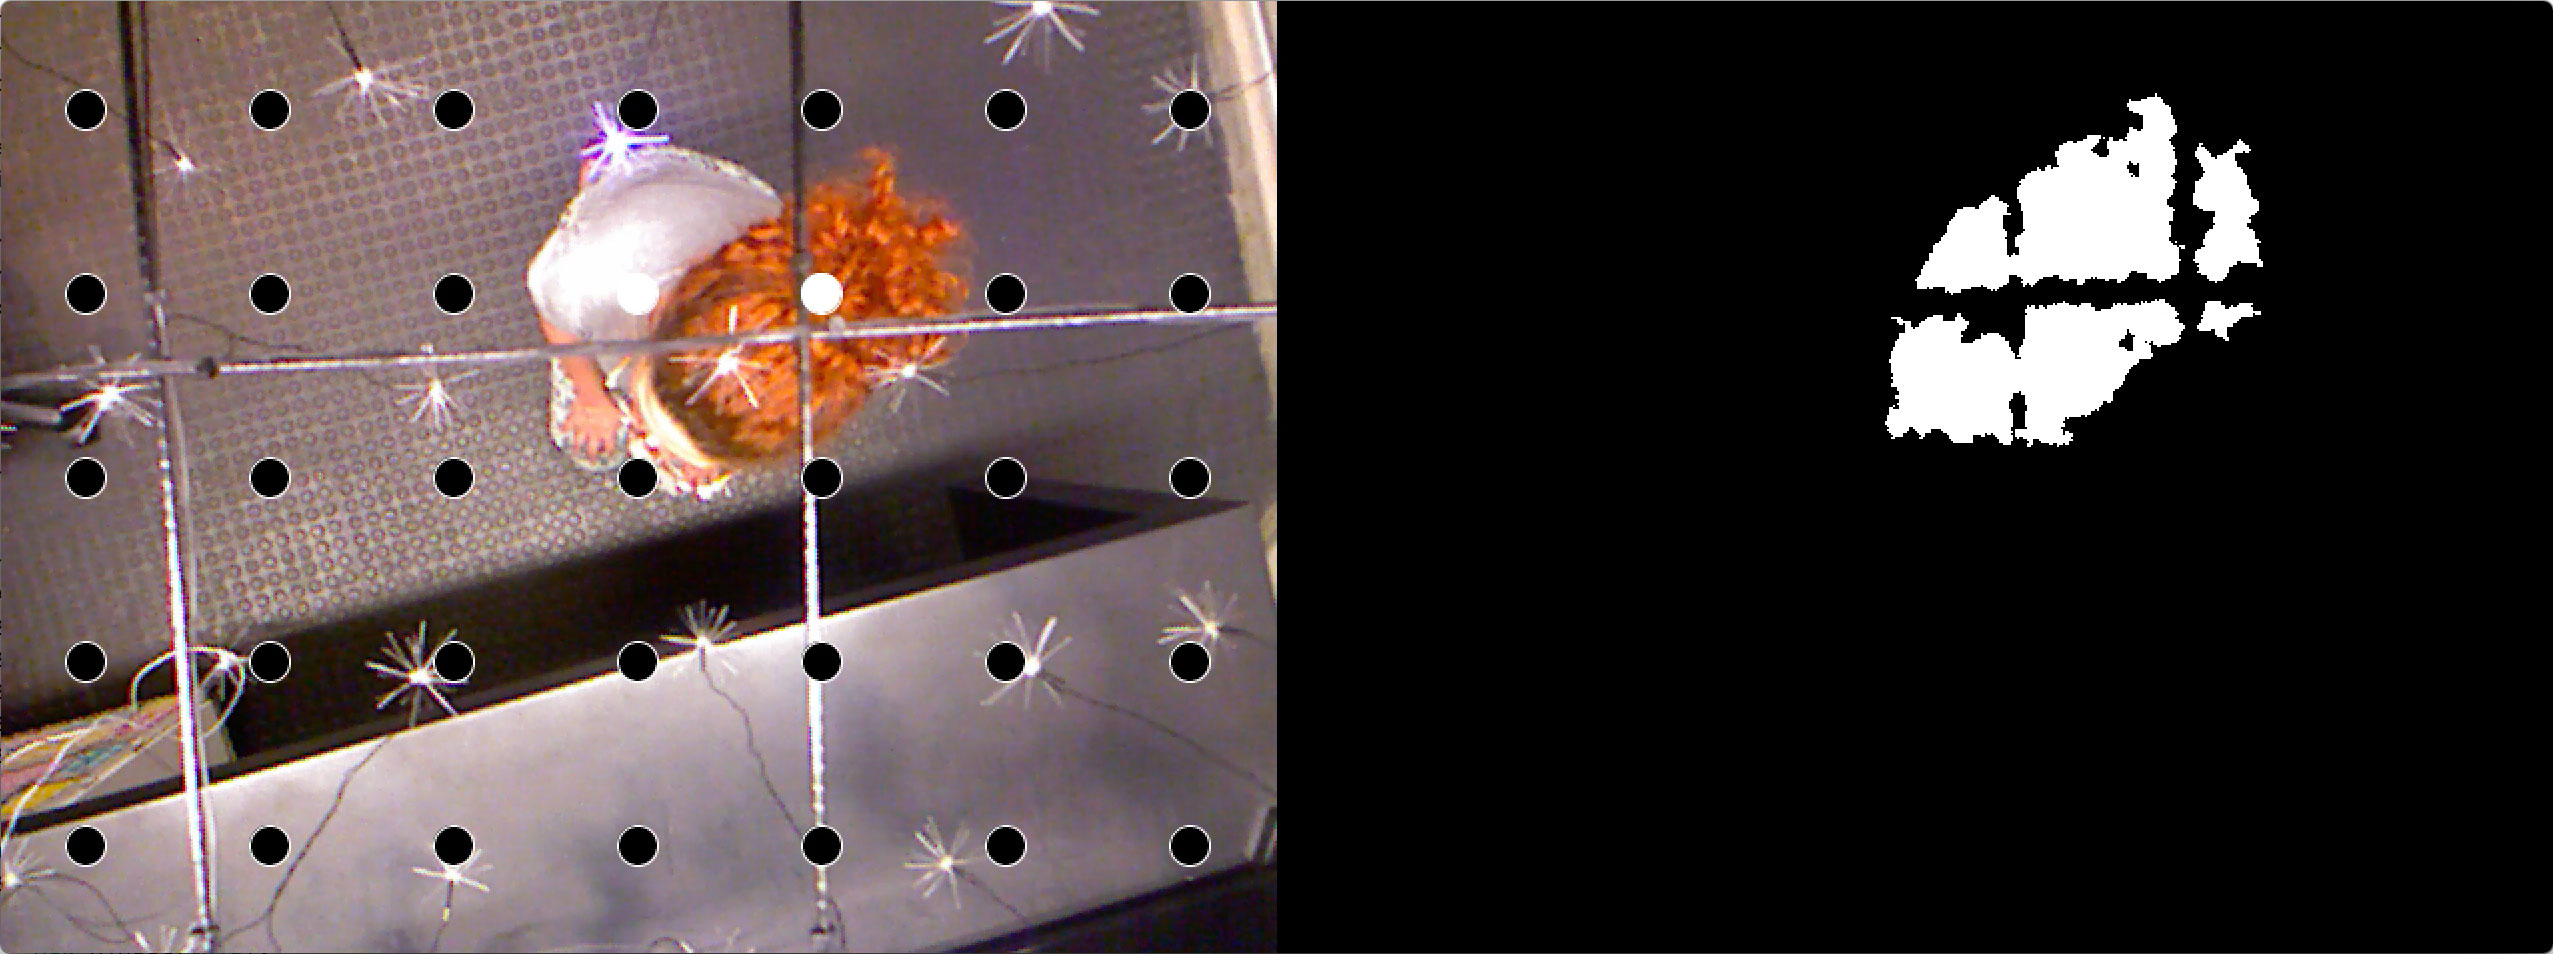
\includegraphics[width=0.8\textwidth]{./04-figuras/script}
    \label{fig:script}
  \end{center}
  \vspace*{-0,9cm}
  \fonte{Elaborada pela autora}\\
\end{figure}

\subsection{\textbf{Dispositivo de saída de dados}}

O Arduino e a malha de LEDs, juntos, formam o dispositivo de saída de dados (\textit{output}) que recebe as informações mapeadas pelo sensor Kinect (entrada ou \textit{input}). Cada LED precisa ser controlado individualmente, por isso optou-se pela utilização do Arduino Mega 2560 que possui 54 entradas/saídas digitais, suficientes para atender a proposta apresentada sem adicionar complexidade ao circuito.


Não foi necessário escrever um \textit{software} para executar no Arduino. Utilizou-se a biblioteca Firmata para servir como ponte de comunicação entre o dispositivo e o computador. Através de um programa fornecido pela mesma e enviado para o microcontrolador foi possível gerenciar, a partir da Processing, todos os recursos disponíveis na placa.

\subsubsection{Circuito}

O circuito montado para execução deste trabalho é relativamente simples. As pernas negativas dos LEDs foram soldadas em um fio conectado na porta \textit{ground} do Arduino, enquanto as pernas positivas foram conectadas à fios e plugadas individualmente em portas digitais. Na figura \ref{fig:breadboard} podemos ver o esquema equivalente a uma linha da matriz de LEDs. As demais são conectadas da mesma maneira e só não foram adicionadas para não poluir a imagem.

\begin{figure}[H]
  \begin{center}
    \caption{Circuito equivalente a uma linha da matriz de LEDs}
    \vspace*{0,2cm}
    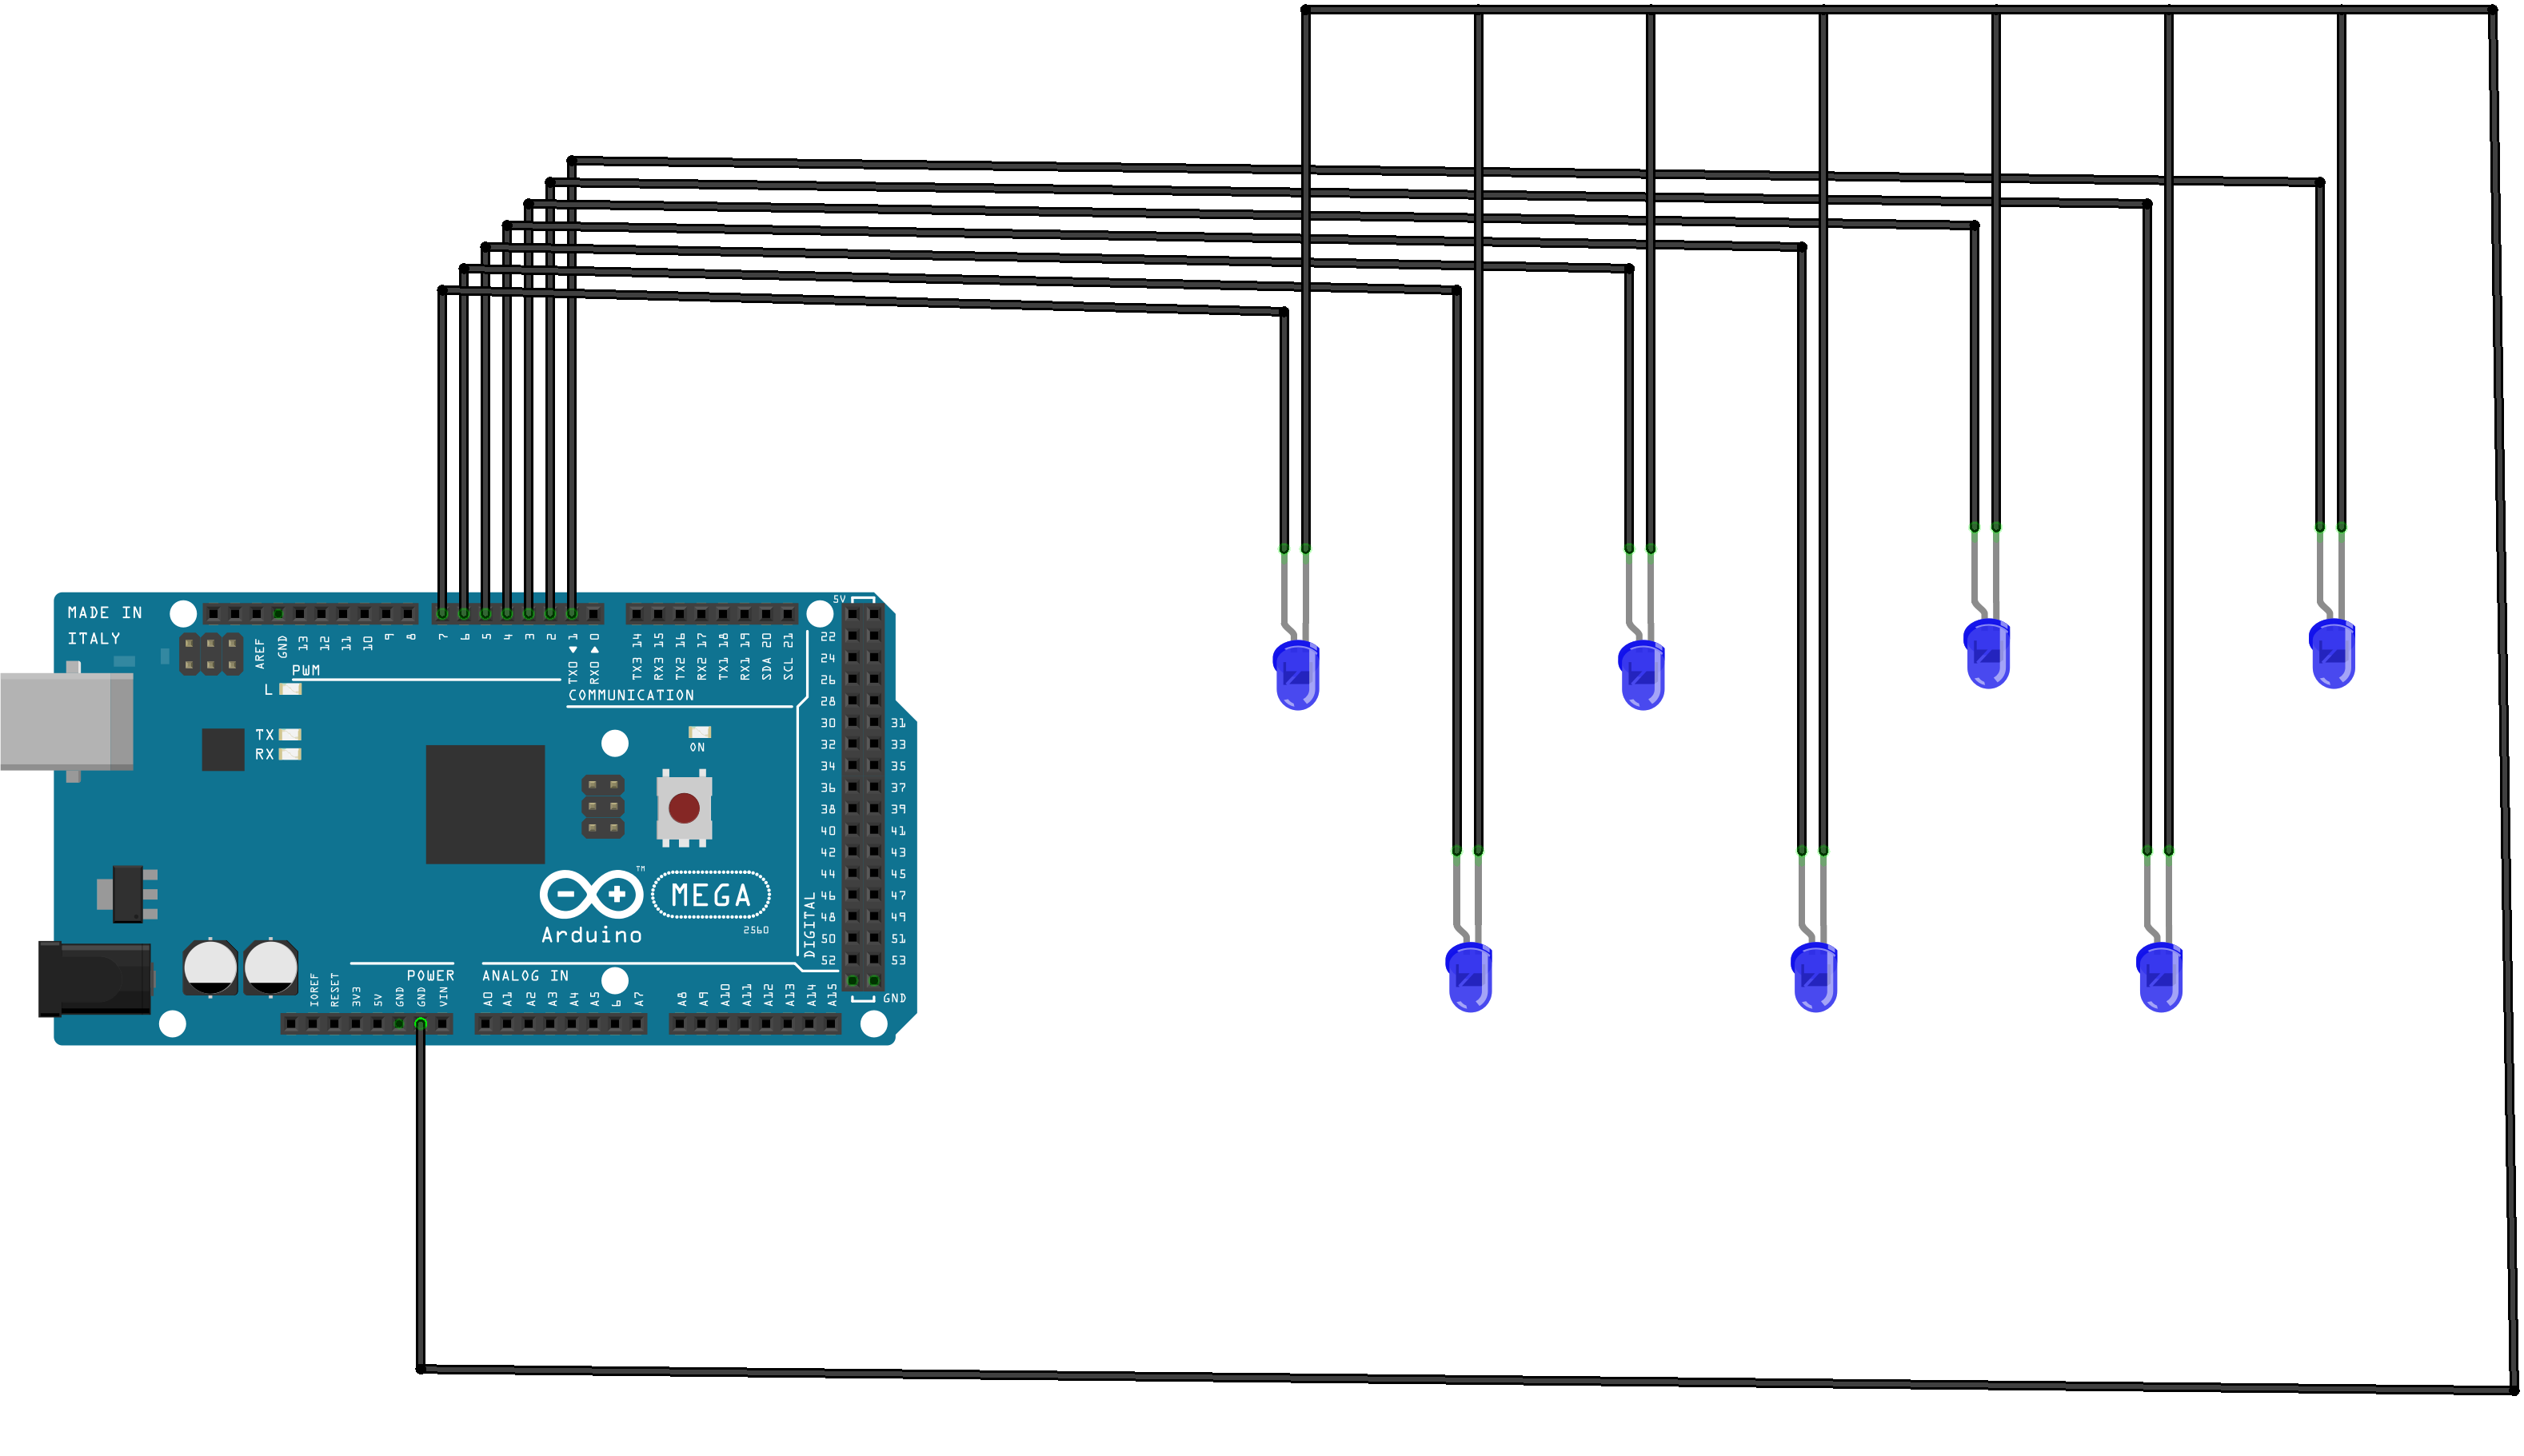
\includegraphics[width=0.8\textwidth]{./04-figuras/breadboard}
    \label{fig:breadboard}
  \end{center}
  \vspace*{-0,9cm}
  \fonte{Elaborada pela autora}\\
\end{figure}

Constatou-se a necessidade de isolamento elétrico e de construir \textit{jumpers} plugáveis na placa. Para isso, alguns materiais foram necessários. Além do próprio LED, pinos metálicos foram utilizados para conectá-lo ao fio e este ao Arduino, \textit{cases} e tubos termoretráteis para isolamento das conexões, bem como a fibra ótica para causar o efeito proposto. O quadro  \ref{quadro:materiais} mostra as quantidades e especificações destes materiais por elemento luminescente.

\begin{quadro}[H]
\caption{\label{quadro:materiais}Materiais utilizados por elemento luminescente}
\begin{center}  
  \begin{tabulary}{1\textwidth}{|L|L|L|}
  
  \hline
  \textbf{Quantidade} & \textbf{Material} & \textbf{Especificação} \\ \hline
  01 peça & LED alto brilho azul & 5 mm \\ \hline
  03 peças & tubo termo retrátil & 1 mm de espessura e 5 cm de comprimento \\ \hline
  01 peça & pino metálico & macho \\ \hline
  01 peça & \textit{case} plástico & -  \\ \hline
  02 peças & pino metálico & fêmea \\ \hline
  40 cm & fibra ótica \textit{side light} & 0.5 mm de espessura em pedaços de aproximadamente 3 cm \\ \hline
  40 cm & fibra ótica \textit{side light} & 0.75 mm de espessura em pedaços de aproximadamente 3 cm \\ \hline
  20 cm & fibra ótica \textit{side light} & 1 mm de espessura em pedaços de aproximadamente 3 cm  \\ \hline
  Tamanho variado & fio & AWG 30 \\ \hline
  \end{tabulary}
\end{center}
\vspace*{-0,7cm}
\fonte{Elaborado pela autora}\\
\end{quadro}


\subsubsection{Malha de LEDs}
\label{sec:malha}

A malha é composta primariamente por uma grade de 120 x 80 centímetros que delimita o espaço da instalação onde o espectador pode interagir com a obra. Como podemos ver na figura \ref{fig:malha}, esta grade possui intersecções a cada 20 centímetros, formando uma matriz de 5 linhas por 7 colunas. Cada intersecção possui um LED preso à ela, somando um total de 35 LEDs dispostos na obra.

\begin{figure}[H]
  \begin{center}
    \caption{Esquema da malha de LEDs}
    \vspace*{0,2cm}
    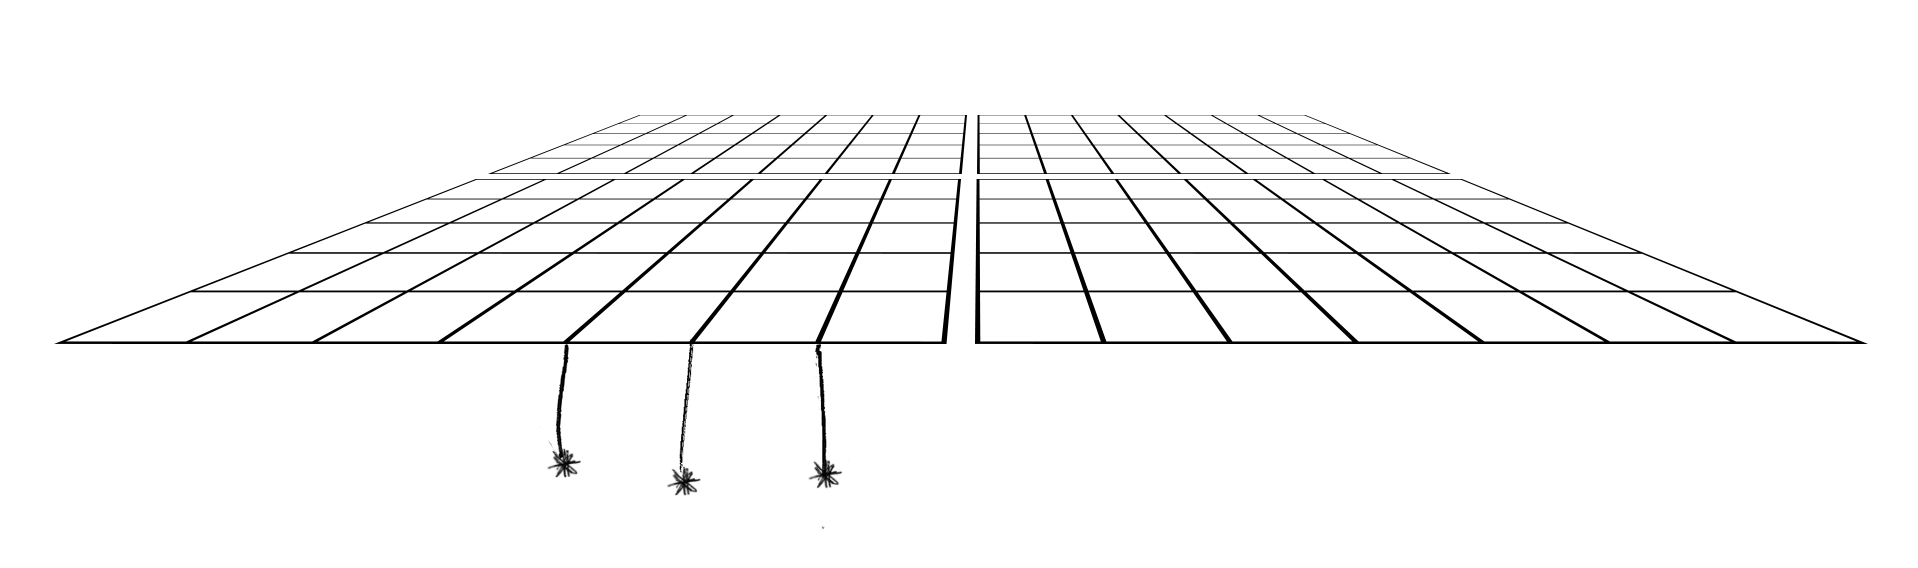
\includegraphics[width=0.8\textwidth]{./04-figuras/malha}
    \label{fig:malha}
  \end{center}
  \vspace*{-0,9cm}
  \fonte{Elaborada pela autora}\\
\end{figure}


Cada LED ocupa uma área na imagem processada pelo sistema computacional e conta com fios de fibra ótica, com emissão de luz lateral, de várias espessuras colados em sua extremidade. Quando o LED acende, a partir da interação com o usuário, a luz é transmitida pela fibra ótica, gerando vários pontos iluminados. Na figura \ref{fig:led_fibra_otica} podemos ver o exemplo de um desses LEDs, sendo que, no primeiro quadro o LED é exibido apagado, no segundo aceso em ambiente com alta luminosidade e, por fim, no terceiro quadro, aceso em ambiente com baixa luminosidade. 

\begin{figure}[H]
  \begin{center}
    \caption{LED com fibra ótica em diferentes condições de luminosidade}
    \vspace*{0,2cm}
    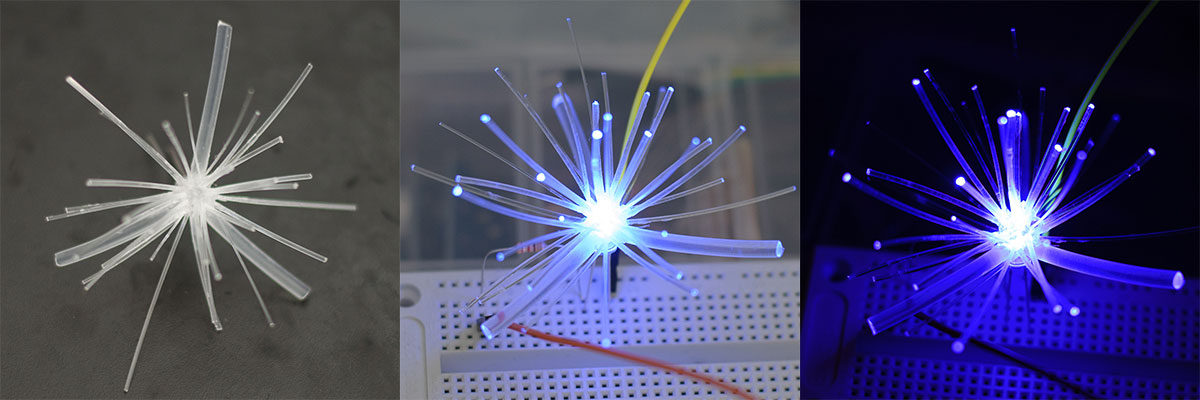
\includegraphics[width=0.8\textwidth]{./04-figuras/led_fibra_otica}
    \label{fig:led_fibra_otica}
  \end{center}
  \vspace*{-0,9cm}
  \fonte{Elaborada pela autora}\\
\end{figure}

A partir da figura \ref{fig:led_fibra_otica} é possível constatar a diferença de exposição em ambientes com distintos graus de luminosidade. Ainda que a luz seja visível ao se observar o LED em um ambiente com alta incidência de luz e, isso viabilize a exposição do trabalho mesmo em condições como esta, se nota uma discrepância considerável quando voltamos nossos olhos para o terceiro quadrante, onde o LED é apresentado em ambiente com baixa luminosidade. A peça ganha destaque e a cor azul se propaga com maior intensidade.

\section{MONTAGEM E INSTALAÇÃO}

A obra foi disposta em um ambiente de laboratório para que fossem realizados testes de funcionamento e iluminação. Na figura \ref{fig:trabalho} podemos ver o resultado em um exemplo de interação com o público. Montada em uma sala com iluminação artificial, a propagação da luz se mostrou adequada mesmo não estando em uma local completamente escuro, o que relativiza a preocupação demonstrada com relação à exposição da obra em um ambiente distinto ao do cubo preto.  
   
\begin{figure}[H]
  \begin{center}
    \caption{Interação com o público}
    \vspace*{0,2cm}
    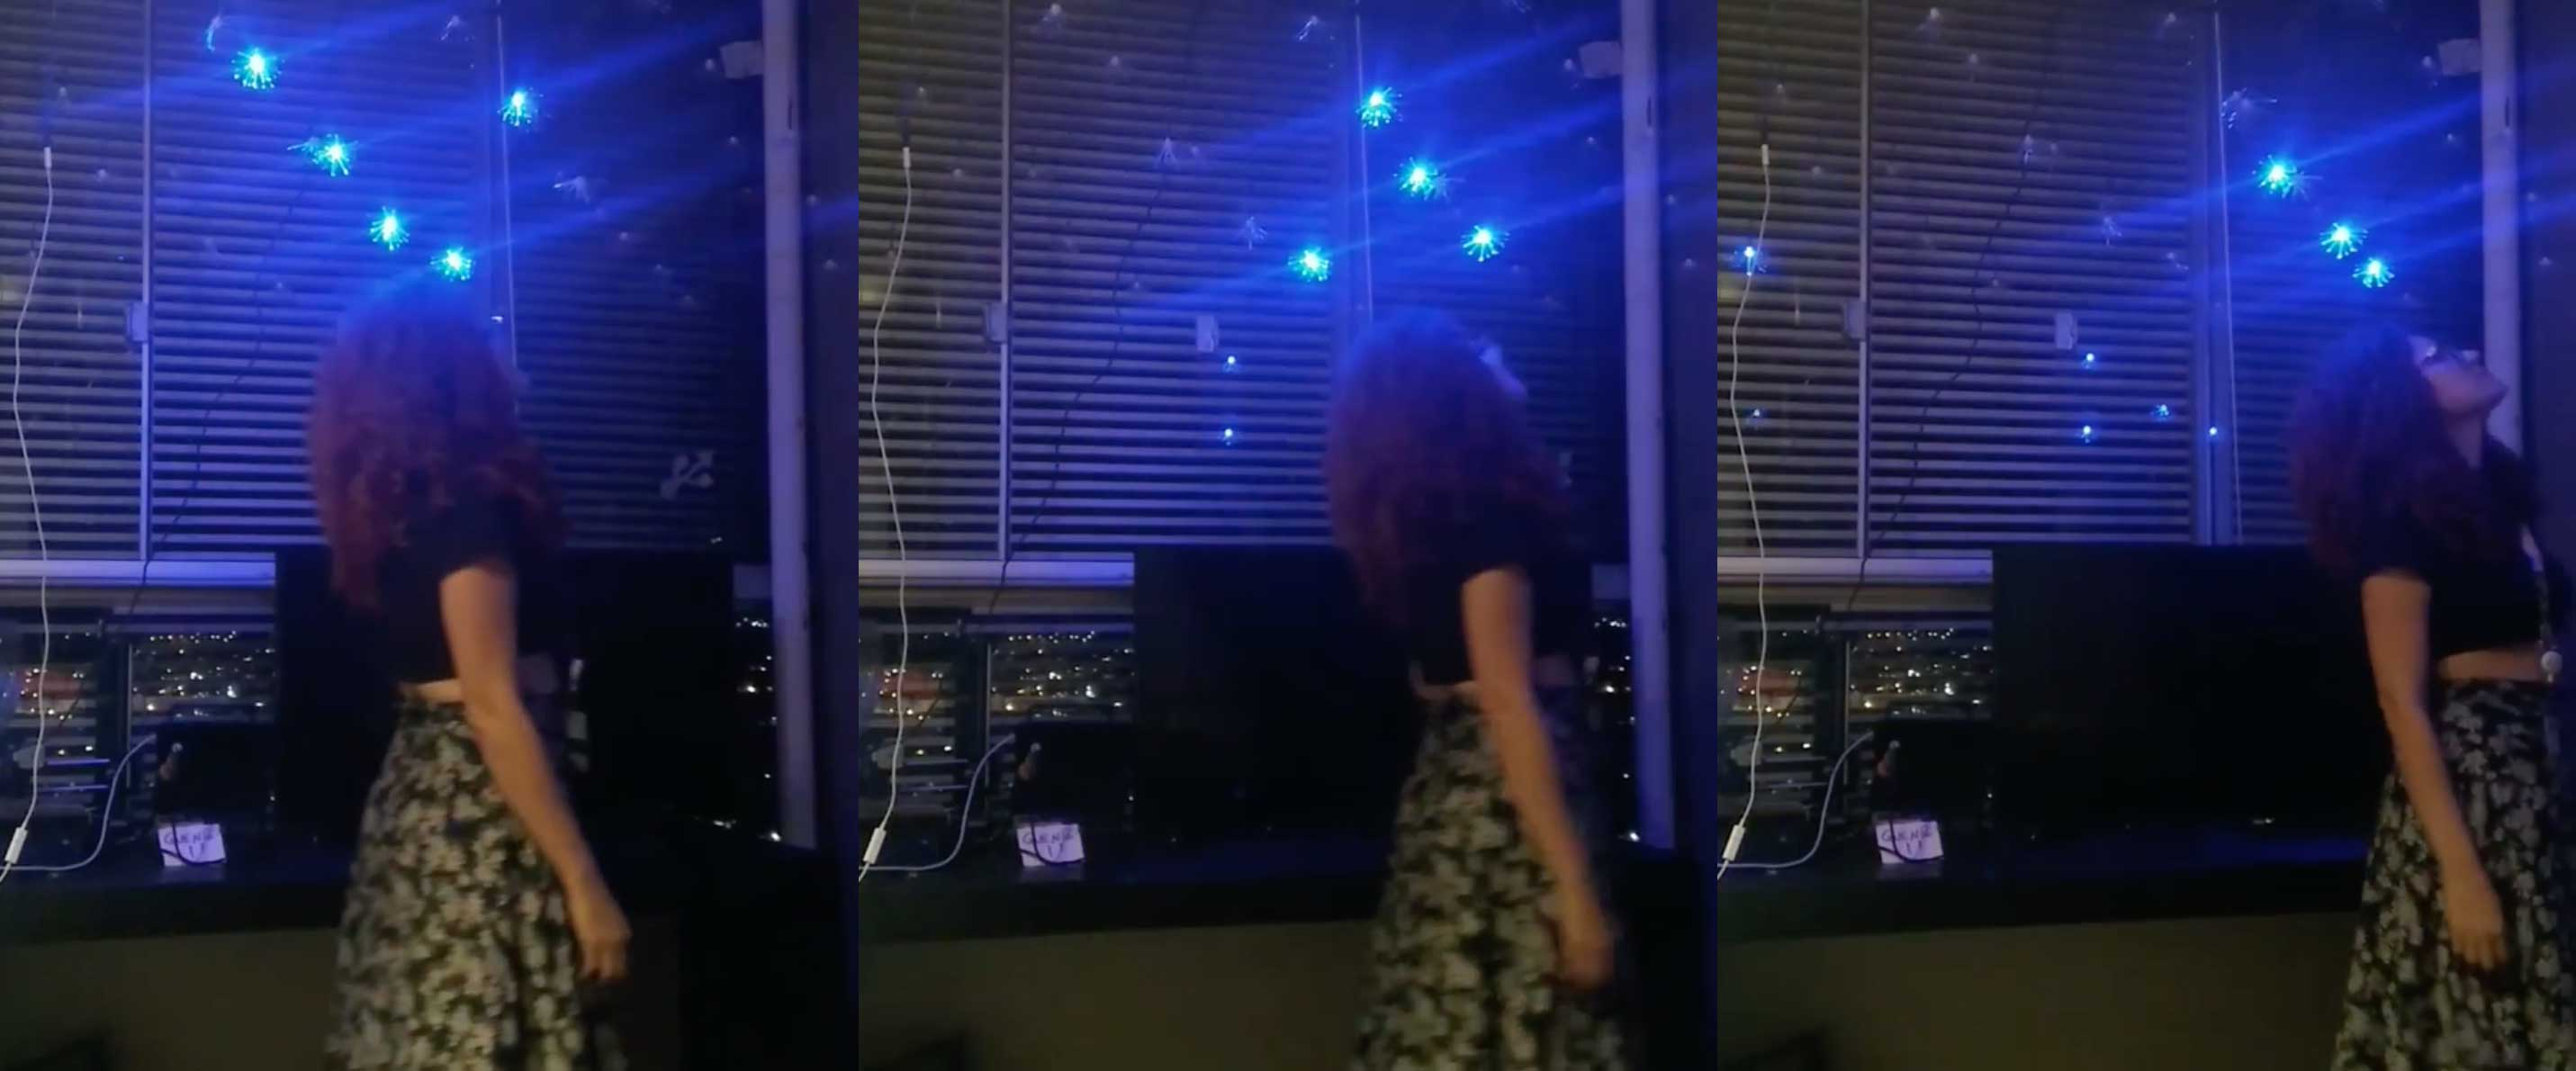
\includegraphics[width=0.8\textwidth]{./04-figuras/trabalho}
    \label{fig:trabalho}
  \end{center}
  \vspace*{-0,9cm}
  \fonte{Elaborada pela autora}\\
\end{figure}

O próximo local de montagem será a pinacoteca Barão de Santo Ângelo, no Instituto de Artes da UFRGS, cuja planta com especificação da área na qual a obra será instalada pode ser vista na figura \ref{fig:pinacoteca}. Com um pé direito de 3,2 metros a pinacoteca oferece as condições necessárias para instalação do trabalho que será fixado no teto através de ganchos. O espaço se trata de um cubo branco, com luz artificial controlada, o que nos dá margem para propor um esquema de iluminação que valorize a obra.

\begin{figure}[H]
  \begin{center}
    \caption{Espaço da instalação na pinacoteca Barão de Santo Ângelo}
    \vspace*{0,2cm}
    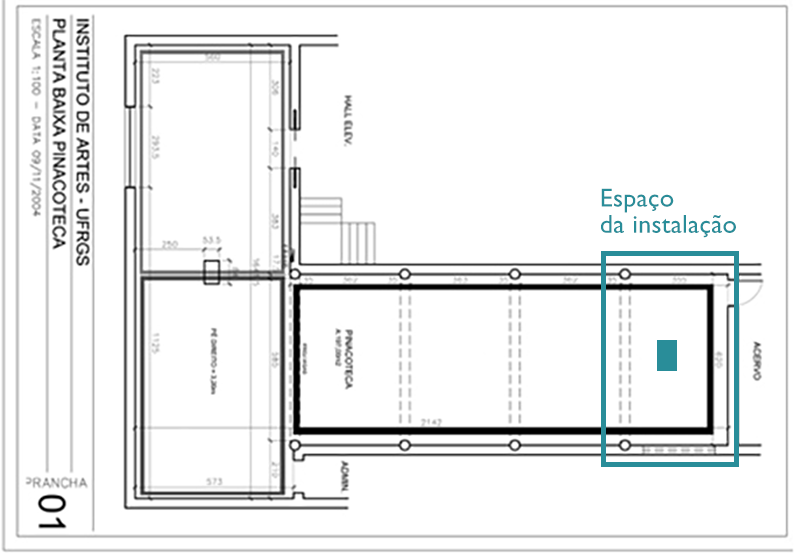
\includegraphics[width=0.8\textwidth]{./04-figuras/pinacoteca}
    \label{fig:pinacoteca}
  \end{center}
  \vspace*{-0,9cm}
  \fonte{Adaptado de https://www.ufrgs.br/institutodeartes}\\
\end{figure}
            	% Citações
    \chapter{CONSIDERAÇÕES FINAIS}

No âmbito deste trabalho, a aplicação da tecnologia e a utilização artística da luz, levou-me à construção de objetos que emanam luz e que, conectados, se completam com a presença do observador. São colocados num espaço com um percurso indefinido, mas com área limitada. Dentro desta área o observador é convidado a explorar seus movimentos e percepções. A experiência confirma a luz como material plástico essencial e a tecnologia como meio para sua execução.

O trabalho realizado é uma amostra da potencialidade do uso da tecnologia na arte e serve como ponto de partida para pesquisas futuras mais aprofundadas. Dando continuidade para a proposta aqui apresentada, algumas variações e otimizações do trabalho foram cogitadas e podem ser aplicadas juntas ou de maneira isolada em trabalhos futuros.

Uma das possibilidades está relacionada ao ganho de escala. No que tem relação com o circuito apresentado, poderiam ser utilizados multiplexadores que permitem aumentar o número de portas digitais do Arduino. Entretanto, a perquisa necessitaria avançar no que diz respeito ao modelo de capturada da presença do espectador no ambiente, dado que a área de abrangência do Kinect é limitada pela altura do local da instalação. A resposta poderia se dar através da triangulação de sensores Kinect ou, talvez, da construção de circuitos mais elaborados utilizando sensores ultrassônicos. Apesar destes sensores terem sido cogitados como uma das possibilidades de implementação dete trabalho, nenhum teste de precisão ou \textit{performance} foi realizado em relação aos mesmos.

Foi possível observar neste experimento que a altura do interator influencia diretamente na fruição da obra. Sendo estabelecida uma média para o posicionamento da grade em relação ao solo, indivíduos mais altos tendem a bater com a cabeça nos LEDs, enquanto crianças menores não conseguem tocar os mesmos. Sendo assim, um possível desdobramento seria permitir uma experiência mais homogênea para espectadores de diferentes estaturas. A figura \ref{fig:malha_futuro} mostra duas possibilidades de variação que foram pensadas para prover esta homogeneidade. À esquerda propõe-se uma variação na forma da grade e, à direita, uma mudança no comprimento dos fios. Ambas as propostas exigem a ampliação da obra para pelo menos o dobro do tamanho apresentado aqui, ainda que ocorra, necessariamente, em apenas um dos eixos. 

\begin{figure}[H]
  \begin{center}
    \caption{Possibilidades de variação da grade}
    \vspace*{0,2cm}
    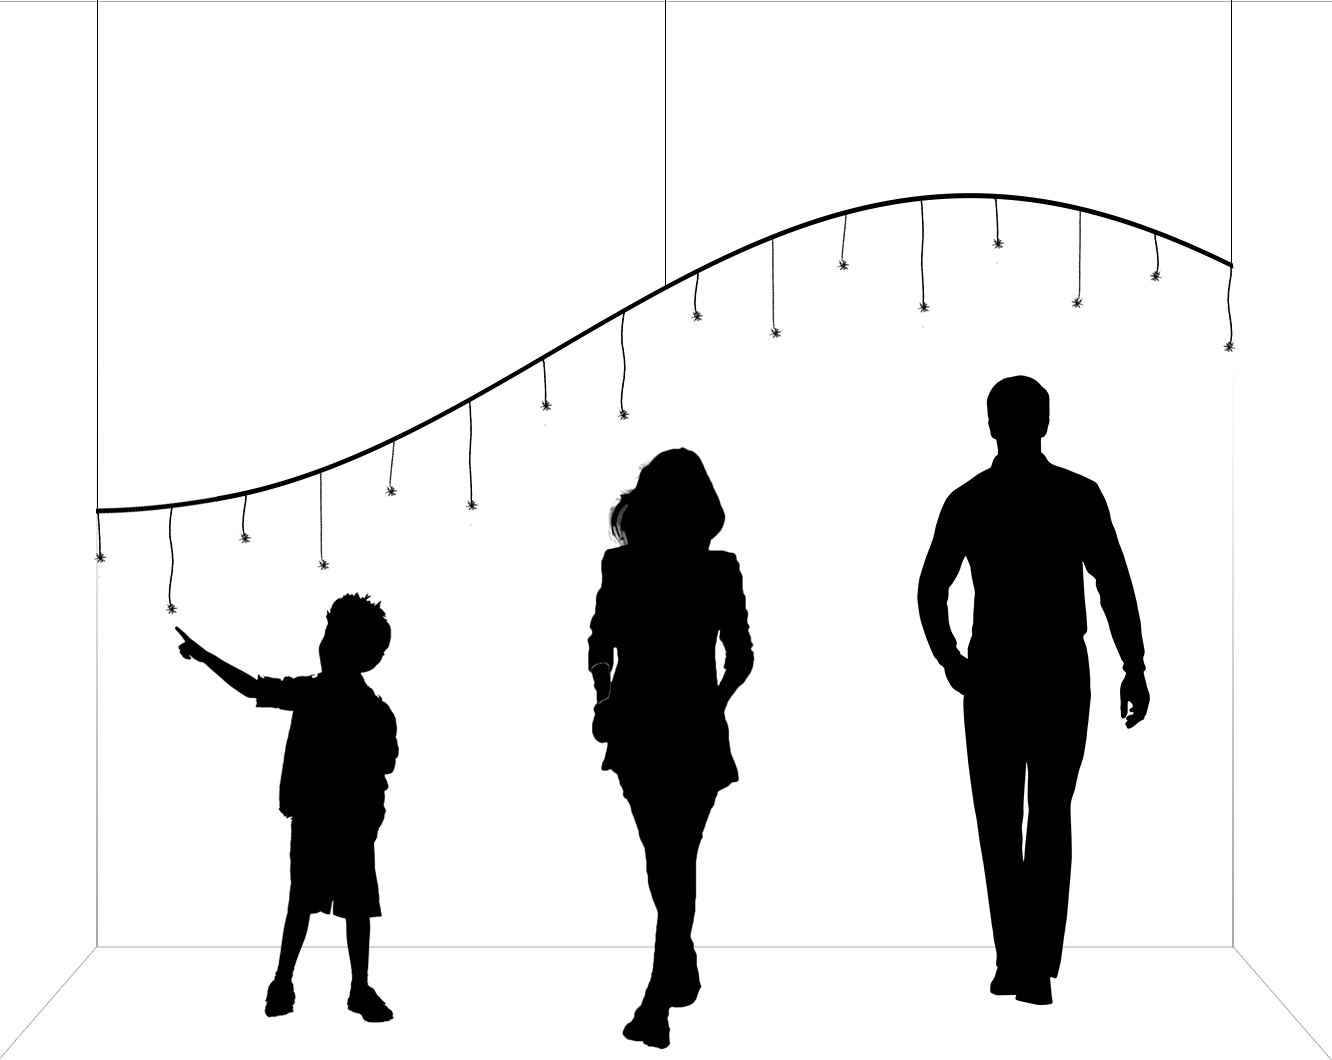
\includegraphics[width=0.8\textwidth]{./04-figuras/malha_futuro}
    \label{fig:malha_futuro}
  \end{center}
  \vspace*{-0,5cm}
  \fonte{Elaborada pela autora}\\
\end{figure}

Outro caminho natural diz respeito a aplicação e otimização de efeitos. Através de alteração do \textit{script} e utilização de portas analógicas seria possível, por exemplo, controlar a intensidade do LED de acordo com a distância do espectador, fazendo-o acender ou apagar gradualmente à medida que o interator se afasta ou se aproxima. Além disso, também poderiam ser trabalhadas a manipulação de cores distintas através da utilização de LEDs RGB, neste caso, as possibilidades de variação dentro do mesmo trabalho são infinitas.

            % Tecnica de referencias 

    % Elementos pós textuais
    \postextual
    %
% Documento: Referências Bibliográficas
%

\bibliography{refbase}    % Geração automática das referências por meio do arquivo 'refbase.bib'
       % Referências
    %%
% Documento: Apêndices
%

\begin{apendicesenv}

\chapter{Como elaborar}

Apêndice é texto ou documento elaborado pelo autor, a fim de
complementar sua argu-mentação, sem prejuízo da unidade nuclear do trabalho. Documentos elaborados por vários au-tores, com um responsável intelectual destacado (organizador, coordenador Elemento opcional.  Deve ser precedido da palavra APÊNDICE, identificado por letras maiúsculas consecutivas, travessão e pelo respectivo título. Utilizam-se letras maiúsculas dobradas, na identificação dos apêndices, quando esgotadas as letras do alfabeto.

\end{apendicesenv}
         % Apêndices
    %%
% Documento: Anexos
%

\begin{anexosenv}

\chapter{Como elaborar}

Anexo é texto ou documento não elaborado pelo autor, que serve de fundamentação, comprovação e ilustração. Elemento opcional. Deve ser precedido da palavra ANEXO, identifi-cado por letras maiúsculas consecutivas, travessão e pelo respectivo título. Utilizam-se letras maiúsculas dobradas, na identificação dos anexos, quando esgotadas as letras do alfabeto.


\end{anexosenv}            % Anexos
    %\printindex                                             % Índice remissivo

\end{document}
